%---------------------------------------------
%	7. Application & Perform of GNN Algorithm
%---------------------------------------------

\chapter{Application of the GNN Algorithm to the TrackML Model}
\label{chapter-7}

This chapter focuses on the application of the GNN algorithm to the Pixel endcap and Pixel barrel regions of the TrackML detector. This chapter is organised as follows. Section \ref{chapter-7-endcap-results} presents the results of the GNN algorithm applied to the Pixel endcap region of the TrackML detector. The performance of the algorithm is evaluated and track reconstruction efficiency metrics are discussed. Section \ref{chapter-7-outlook} presents preliminary results and challenges faced when applying the GNN algorithm onto the full Pixel detector of the TrackML geometry, including the barrel region. Potential software optimisations and other approaches explored are also discussed, followed by several improvements that would be necessary to implement within the GNN algorithm in order for it to be considered for proper online usage for track reconstruction in particle detectors.



\section{Pixel Endcap Results}
\label{chapter-7-endcap-results}


\subsection{Performance Evaluation on Volume 7}
\label{performance-eval-endcap-vol-7-start}

The GNN algorithm is first applied to volume 7 of the TrackML detector model, by isolating the left Pixel endcap. The geometry in the endcap consists of parallel silicon layers and is the simplest part of the detector to begin reconstruction. An example TrackML simulated event shown in volume 7 can be seen in Figure \ref{fig:trackml-results-endcap-nodes-sim}.

\begin{figure}[htbp!] 
    \centering
    \subfloat[$x$-$y$ plane view]{%
        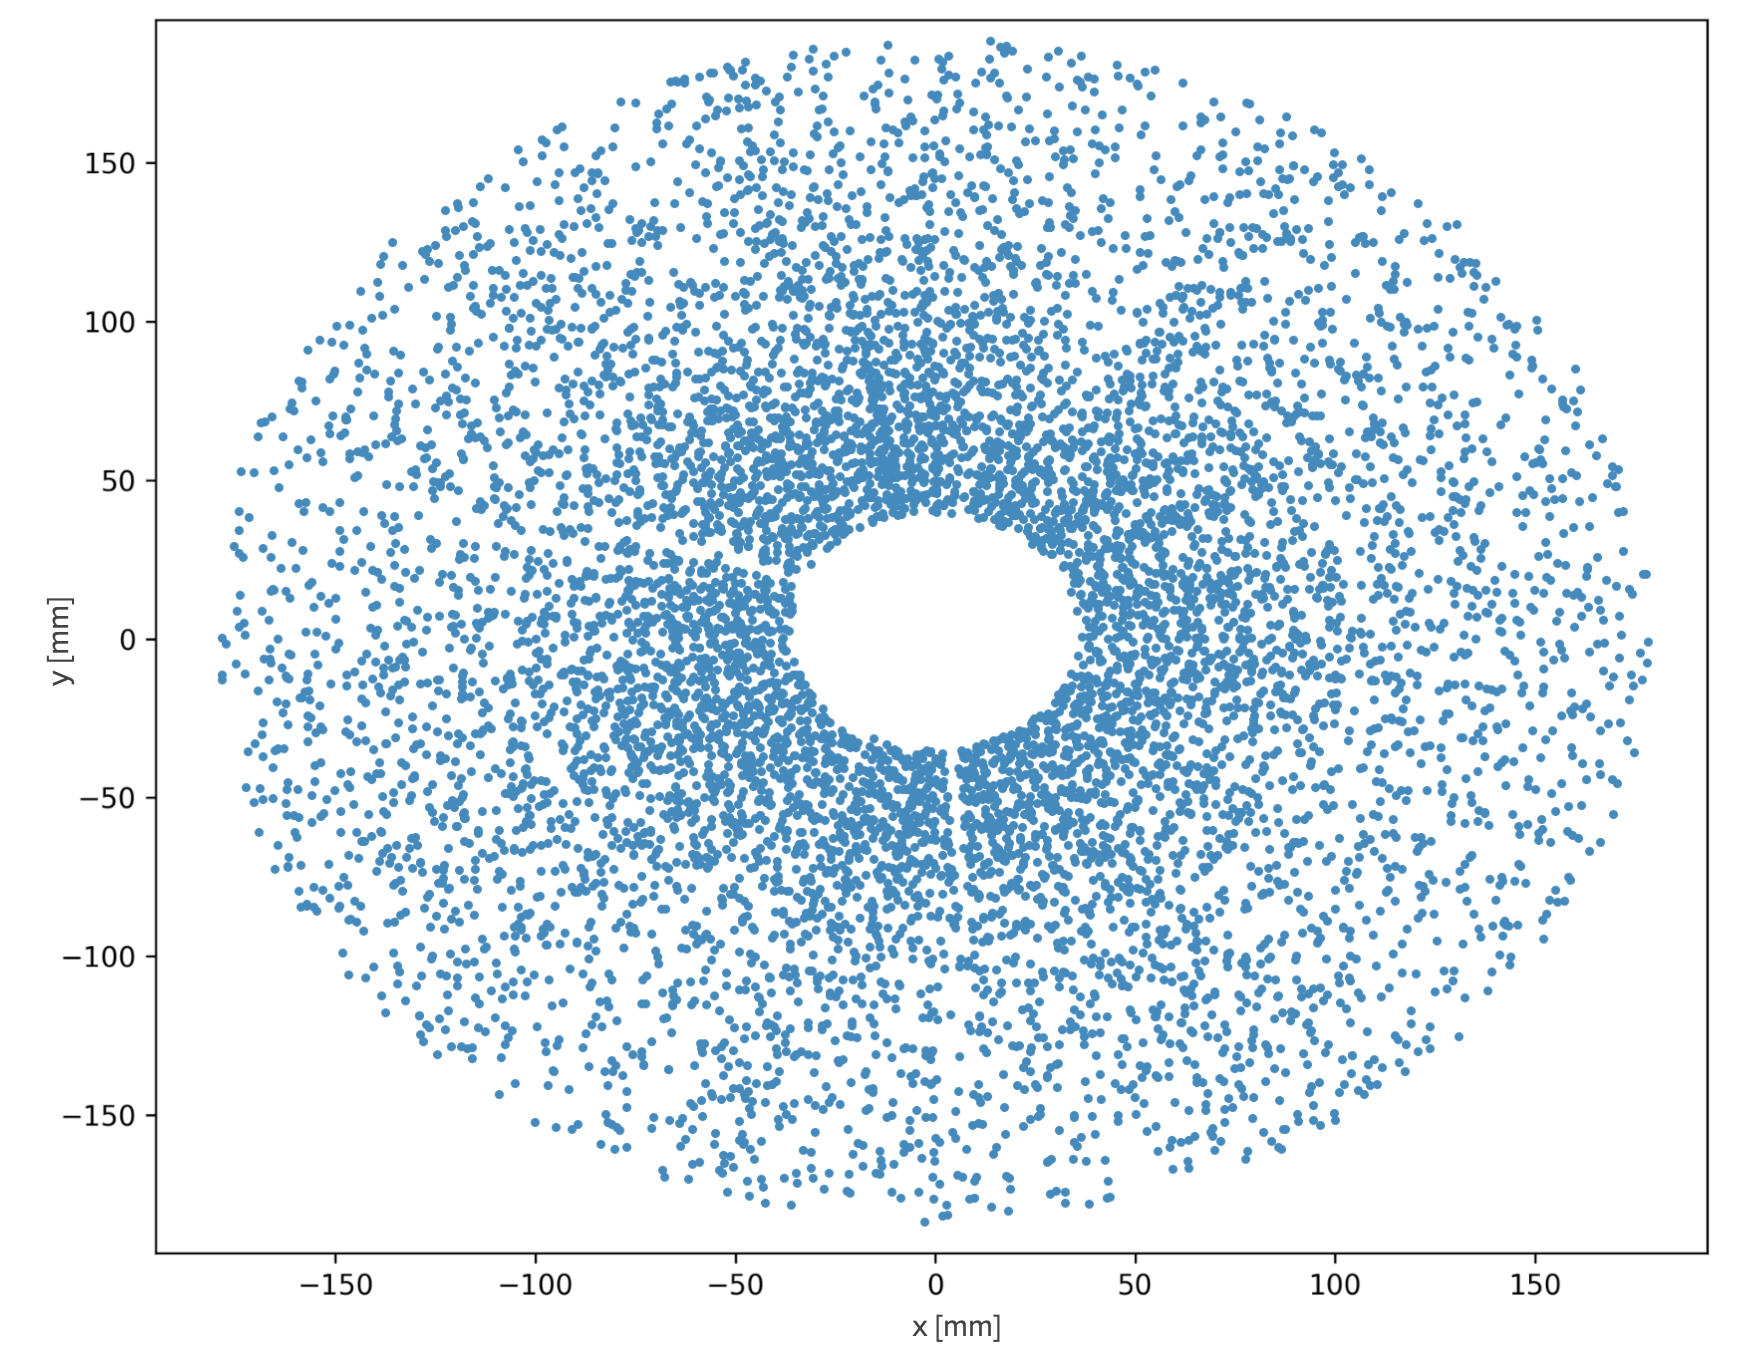
\includegraphics[width=0.50\linewidth]{images/7-results/trackml-endcap-nodes-xy.png}%
        \label{fig:endcap-trackml-sim-xy}%
        }%
    \hfill%
    \subfloat[$r$-$z$ plane view]{%
        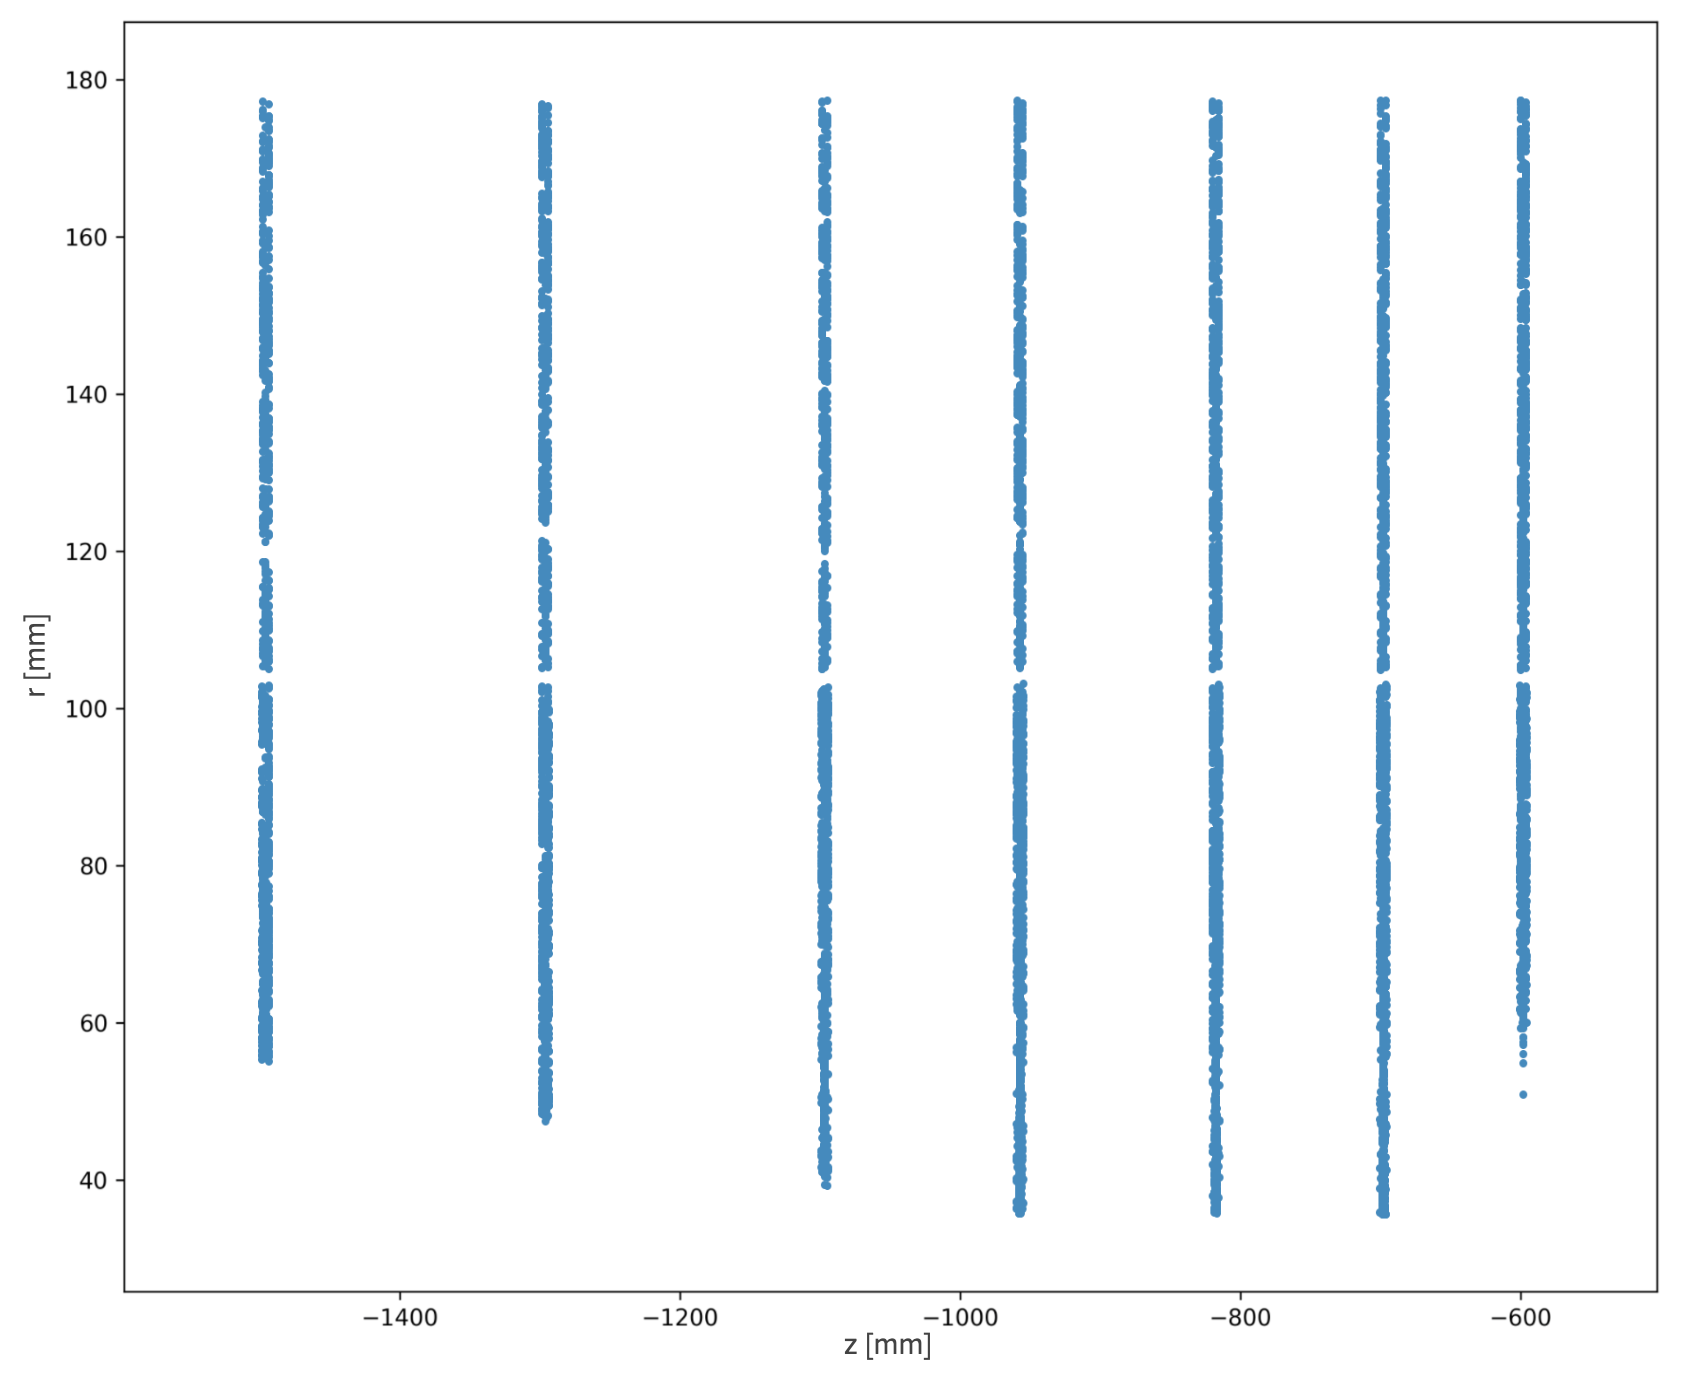
\includegraphics[width=0.48\linewidth]{images/7-results/trackml-endcap-nodes-rz.png}%
        \label{fig:endcap-trackml-sim-rz}%
        }%
    \caption{Event simulation of the TrackML detector isolating volume 7.}
    \label{fig:trackml-results-endcap-nodes-sim}
\end{figure}


The graph network is constructed using 9835 nodes located in volume 7 from a simulated TrackML event and 18,184 predicted edges using the FASTrack algorithm \cite{Dmitry-fasttrack-addtest}, as described in Section \ref{chapter-6-data-prep}. The FASTack algorithm uses several cuts on track parameters when the graph segments are generated. For this particular test the following cut was used: $p_{\text{T}} \ge 150$ MeV. Using the same generated graph, this cut was then increased to $p_{\text{T}} \ge 1$ GeV. Track state estimates, $X_{ij}$, are constructed using the model as described in Section \ref{constructing-track-states}. Figure \ref{fig:trackml-results-endcap-extracted} illustrates the extracted track candidates post Stage 1 of application of the GNN algorithm, where 1054 track candidates were successfully extracted. Figure \ref{fig:trackml-results-endcap-extracted-v2} shows the extracted track candidates post Stage 2, where a further 265 candidates were extracted.

\begin{figure}[htbp]%
    \centering
    \subfloat[\centering $x$-$y$ plane view]{{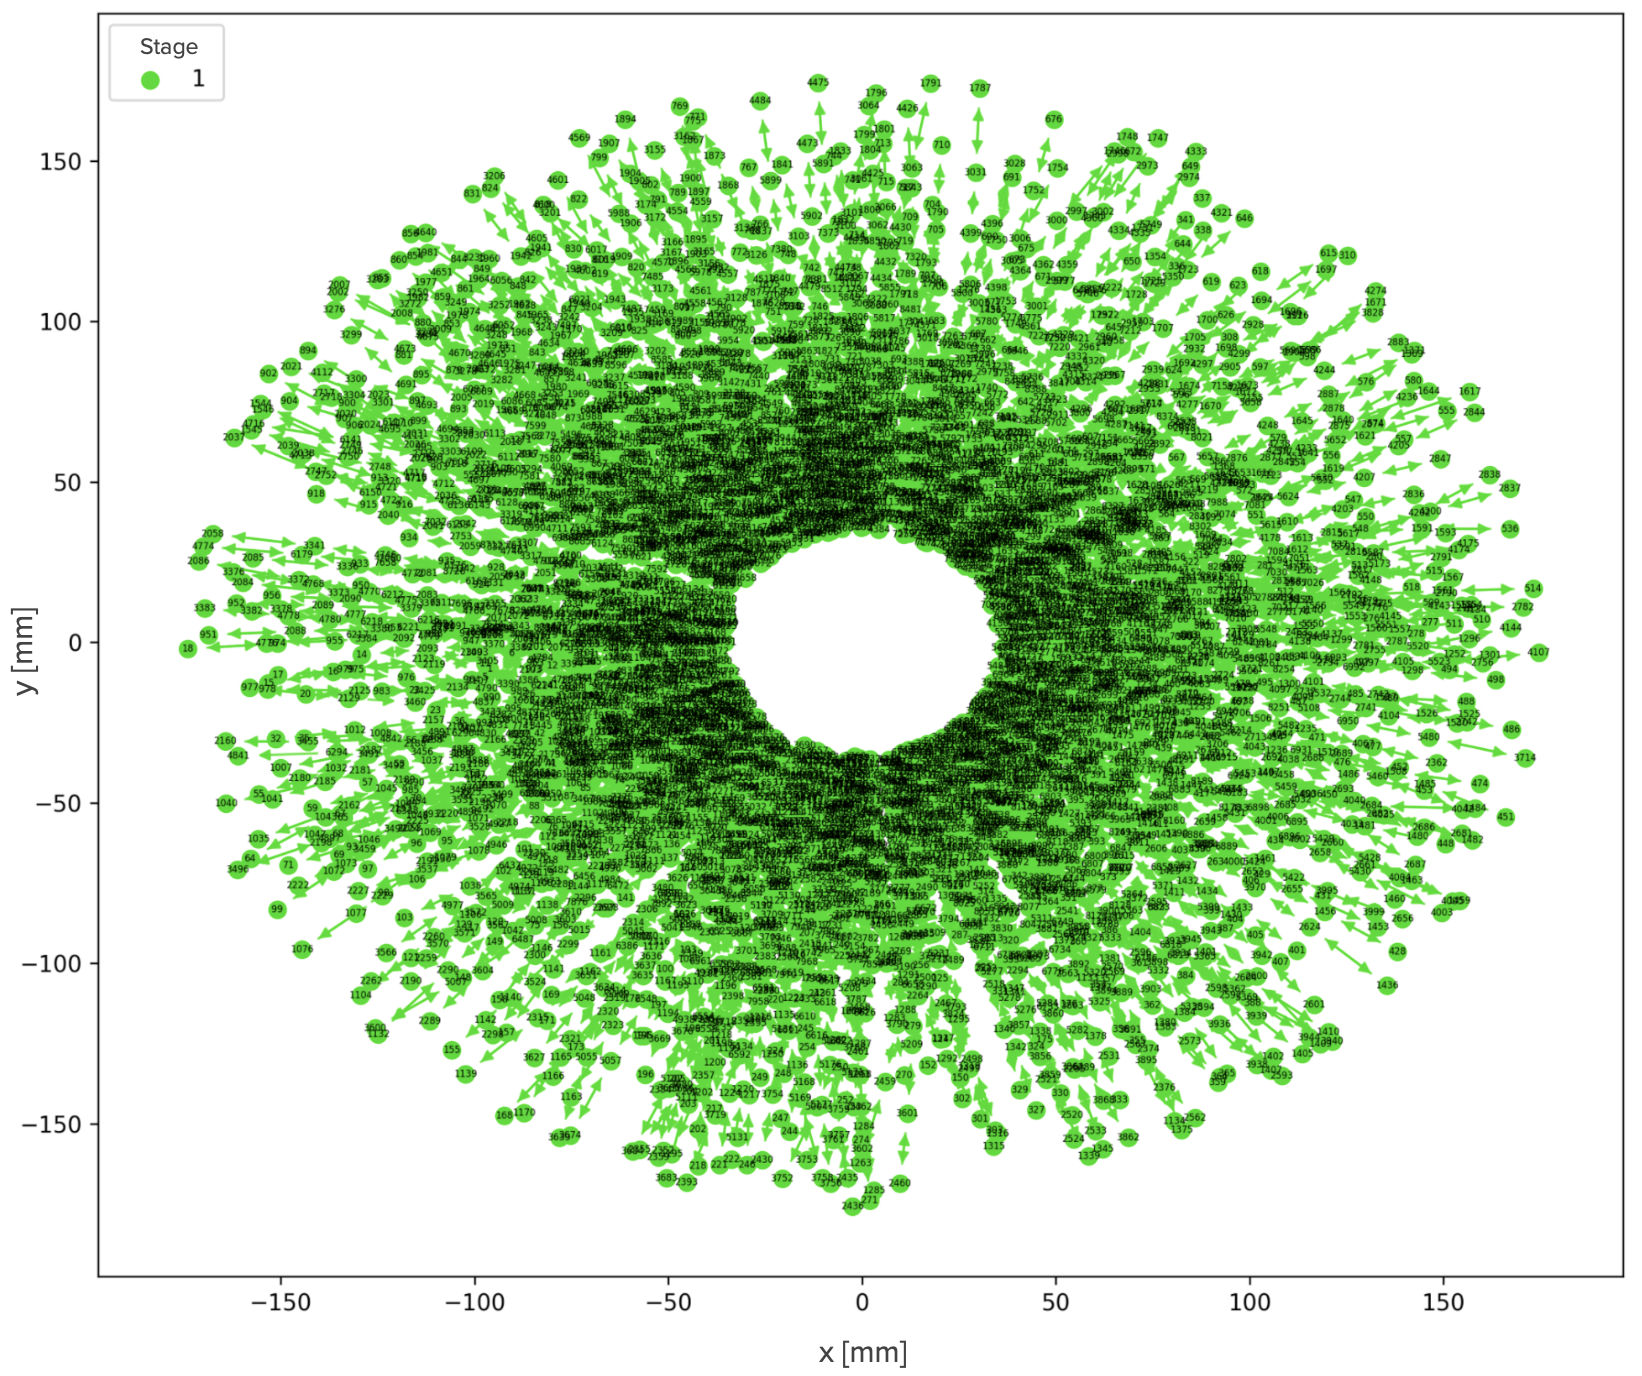
\includegraphics[width=11.5cm]{images/7-results/trackml-endcap-extracted-xy.png} } \label{fig:endcap-trackml-extracted-xy}}%
    \hfill
    %\qquad
    \subfloat[\centering $r$-$z$ plane view]{{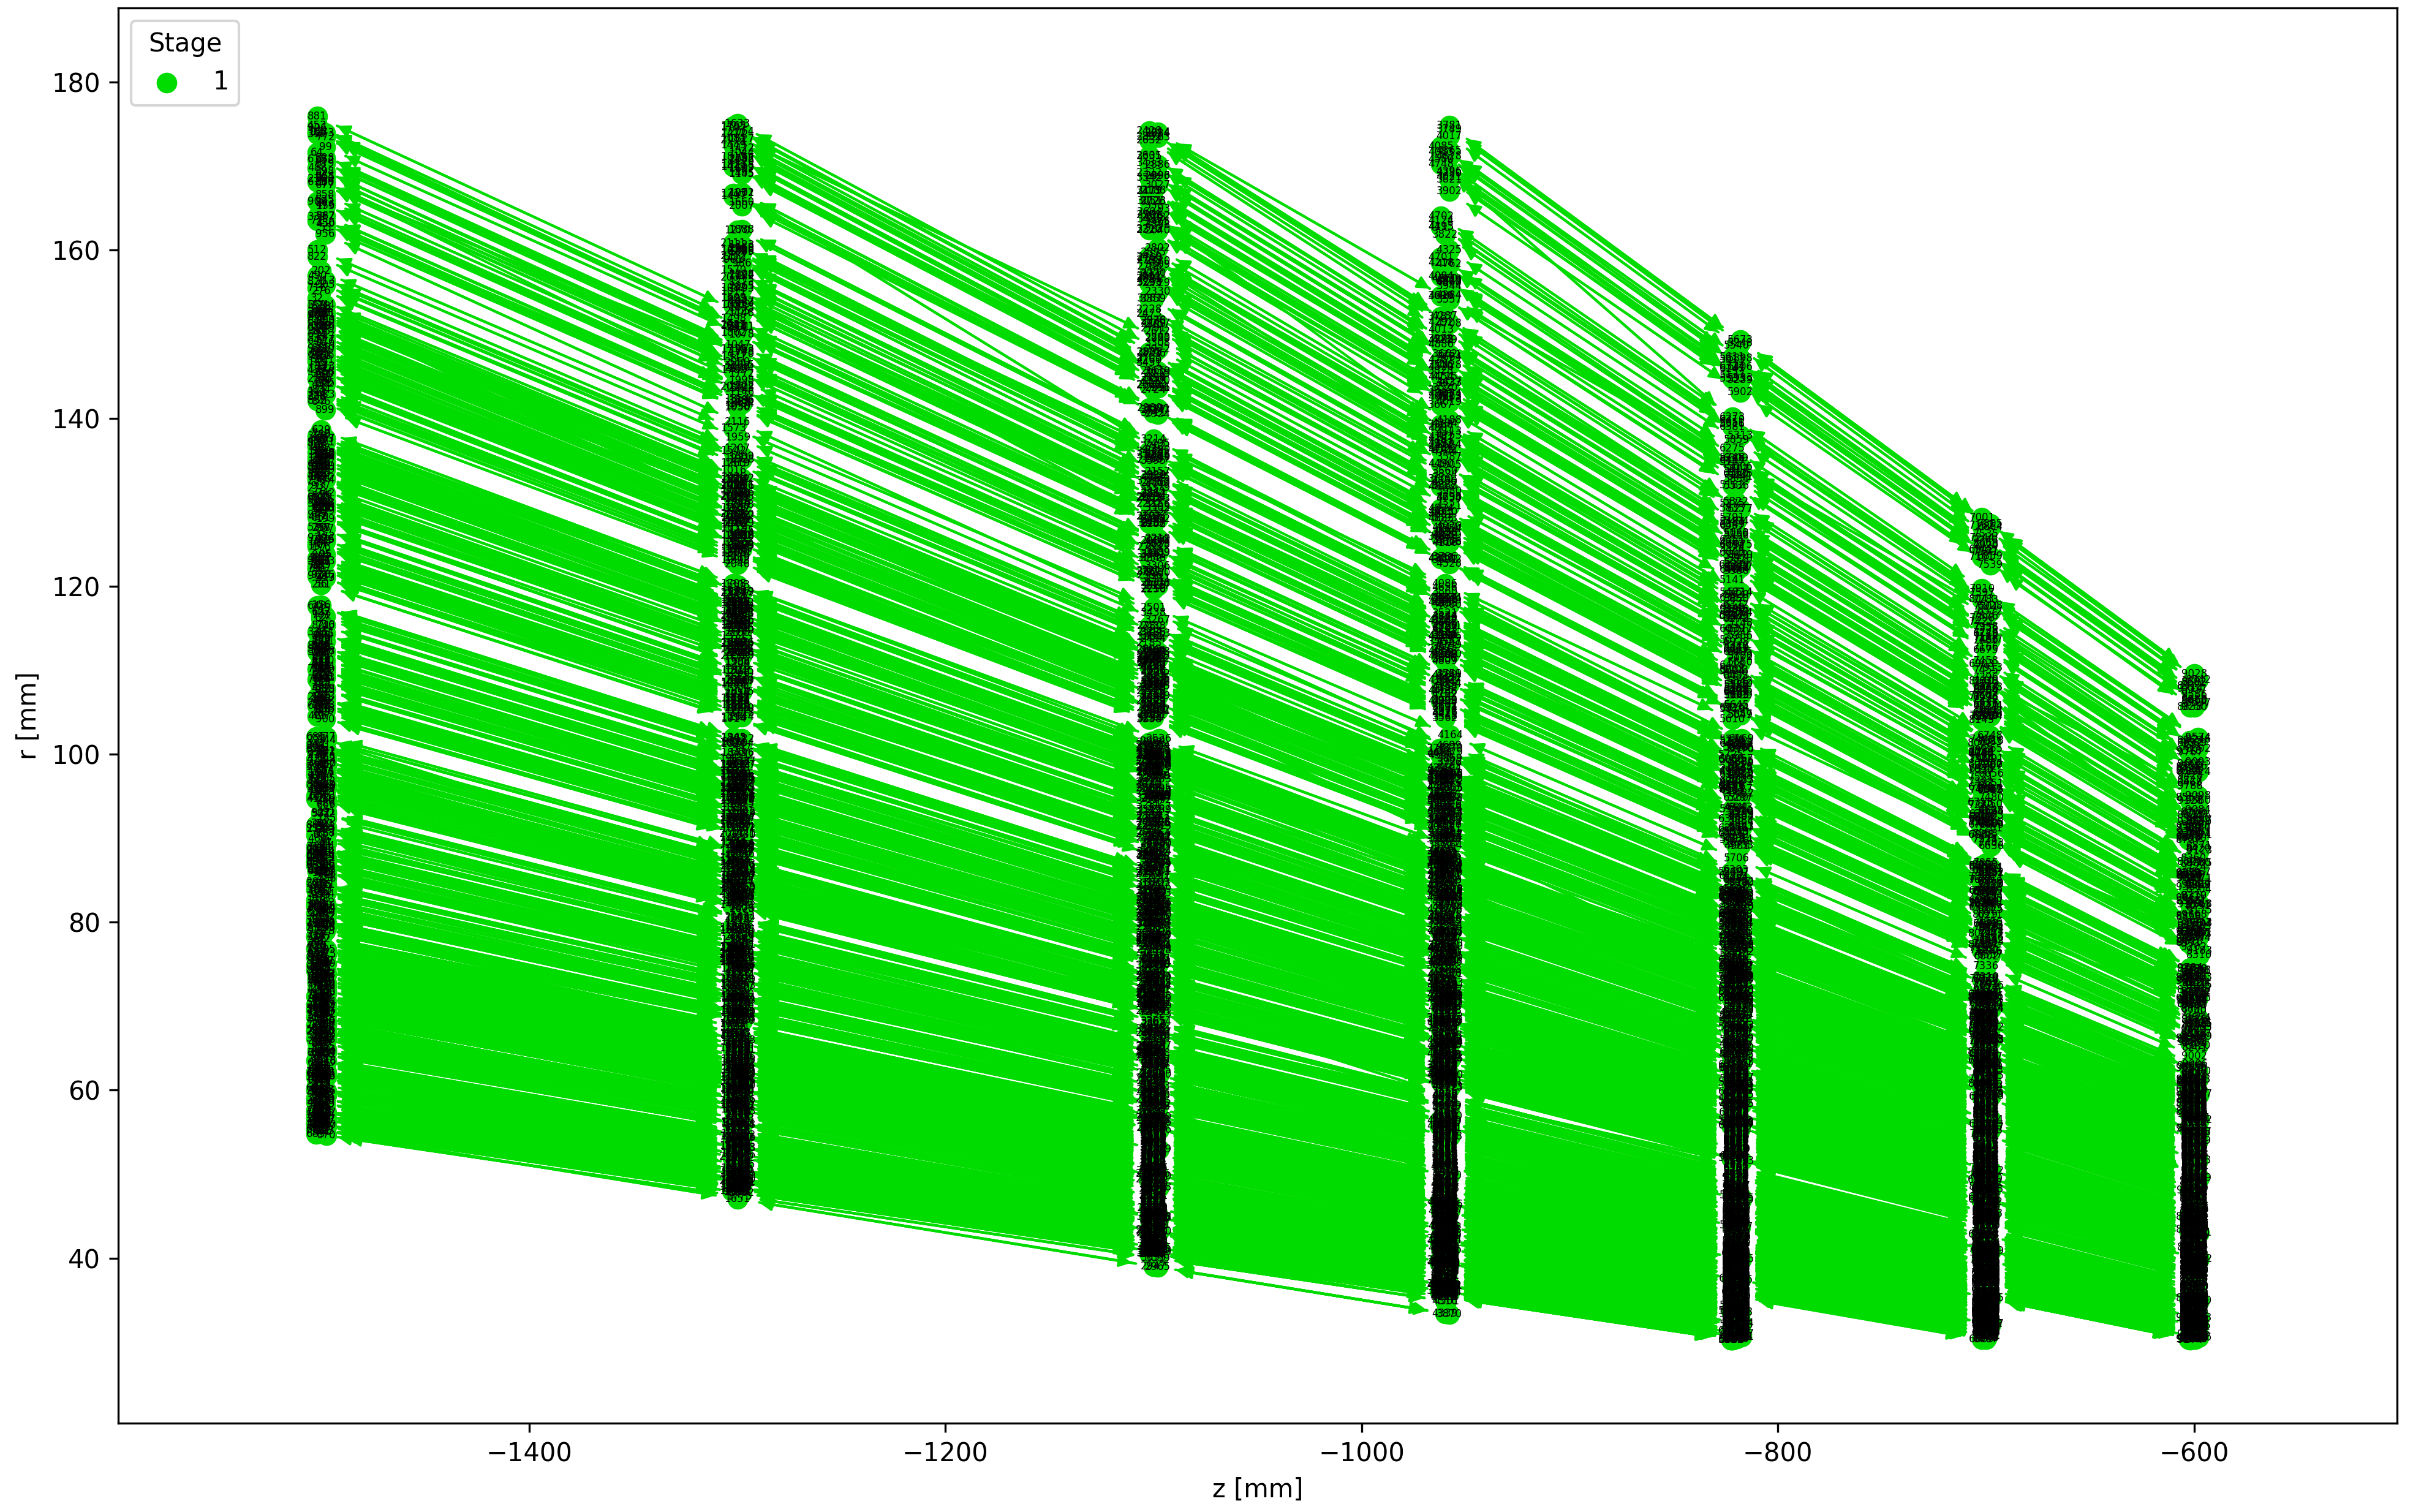
\includegraphics[width=13.5cm]{images/7-results/trackml-endcap-extracted-rz.png} } \label{fig:endcap-trackml-extracted-rz}}%
    \caption{Extracted track candidates post Stage 1 of the GNN algorithm applied to the left Pixel endcap (volume 7) of a simulated TrackML detector event, shown from the view of the a) $x$-$y$ plane and b) $r$-$z$ plane. }%
    \label{fig:trackml-results-endcap-extracted}%
\end{figure}

\begin{figure}[htbp]%
    \centering
    \subfloat[\centering $x$-$y$ plane view]{{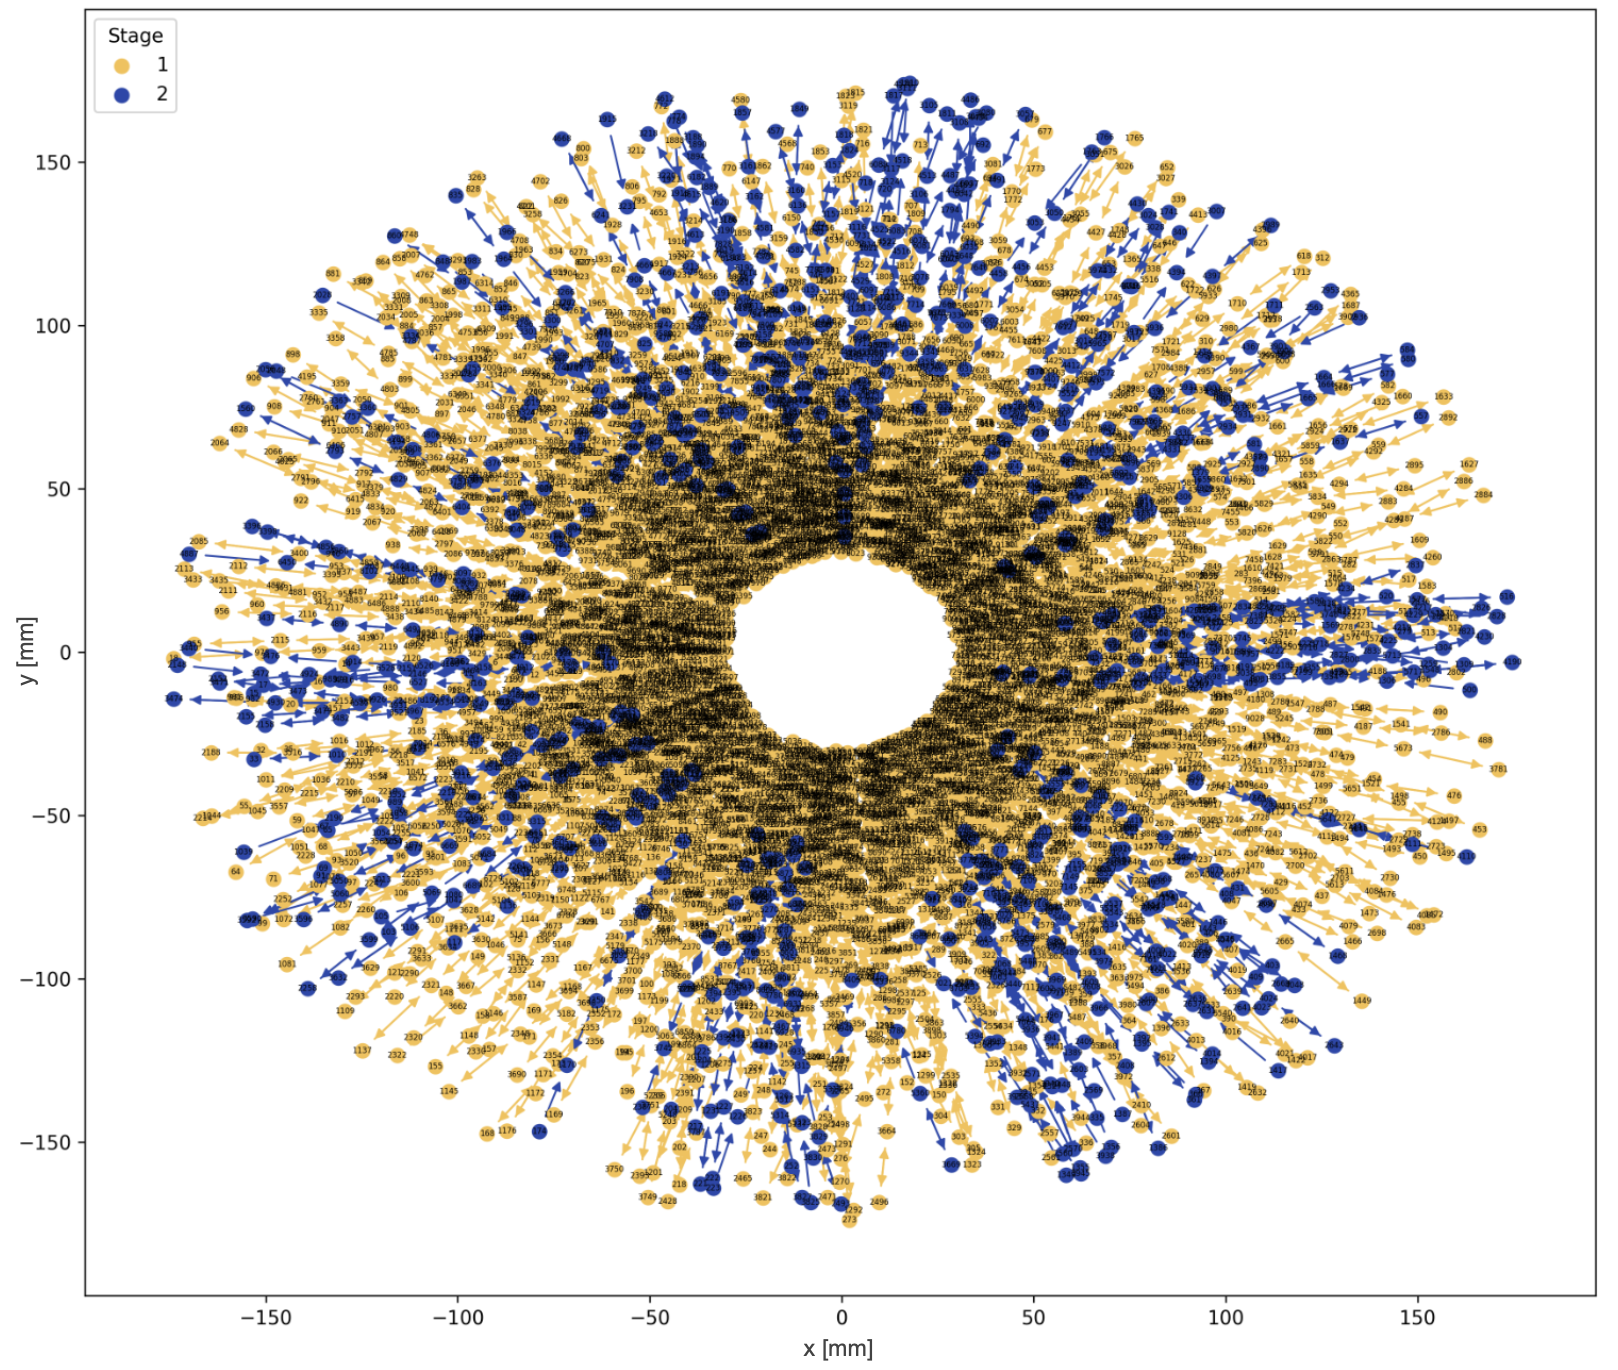
\includegraphics[width=11.5cm]{images/7-results/trackml-endcap-extracted-xy-v2.png} } \label{fig:endcap-trackml-extracted-xy-v2}}%
    \hfill
    %\qquad
    \subfloat[\centering $r$-$z$ plane view]{{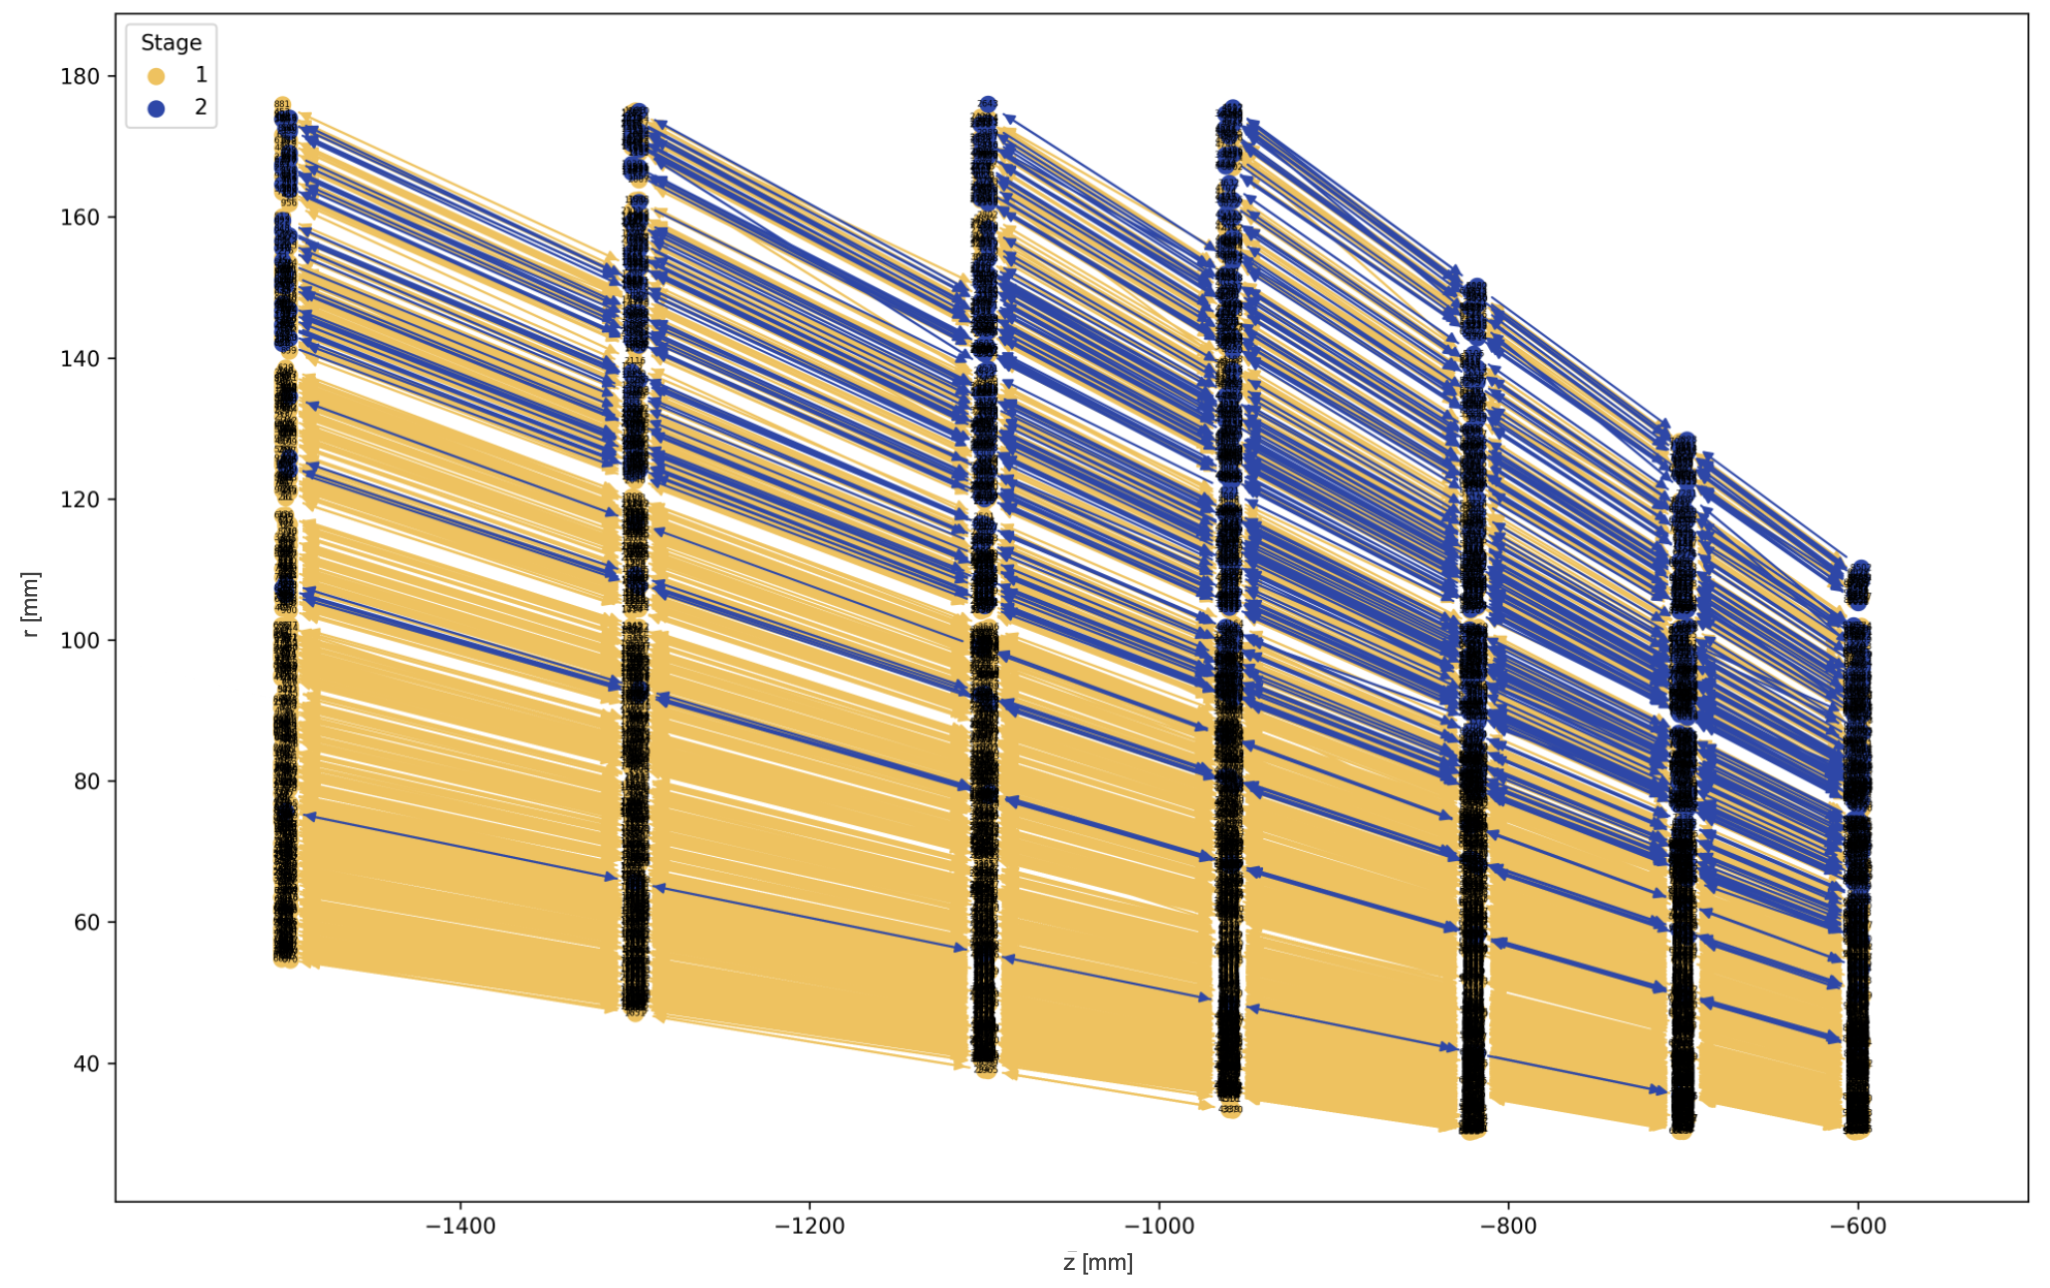
\includegraphics[width=14cm]{images/7-results/trackml-endcap-extracted-rz-v2.png} } \label{fig:endcap-trackml-extracted-rz-v3}}%
    \caption{Extracted track candidates post Stage 1 and 2 of the GNN algorithm applied to the left Pixel endcap (volume 7) of a simulated event of the TrackML detector model, shown from the view of the a) $x$-$y$ plane and b) $r$-$z$ plane.}%
    \label{fig:trackml-results-endcap-extracted-v2}%
\end{figure}

It is clear to see from Figures \ref{fig:endcap-trackml-extracted-xy} and \ref{fig:endcap-trackml-extracted-xy-v2} that track candidates are extracted uniformly within the endcap across all $ 0^{\circ} \leq \phi \leq 360^{\circ}$ during Stage 1 of the GNN algorithm. This is as expected due to the rotational symmetry of the detector in the transverse plane. During Stage 2, we observe the majority of track candidates which are extracted are located at a larger $\theta$ to the $z$-axis (smaller $\eta$). This may be an indication of regions of greater node and edge density, and hence there is a greater proportion of ambiguities to resolve.

The proportion of nodes removed from the main graph network during Stage 1 and Stage 2 were 68\% and 14\% respectively, leaving 18\% of nodes to be further processed. On application of Stage 3 of the GNN algorithm (a further GMR), no additional track candidates were extracted.

% beginning: 9835 nodes
% post stage 1: 3165 nodes
% post stsge 2: 2123 nodes

\subsection{Confusion Matrices}
\label{confusion-matrices-endcap-trackml}

An \textit{outlier edge} is defined to be an edge where its nodes do not belong to the same truth track (truth 1). A \textit{good edge} is defined to be an edge where its nodes do belong to the same truth track (truth 0). The following confusion matrices depict the prediction summary of the GNN algorithm onto the TrackML simulated event, where predicted class 1 indicates the prediction of outlier edges with respect to MC truth and predicted class 0 indicates the prediction of good edges to remain active in the network. The confusion matrix for Stage 1 of the GNN algorithm applied to volume 7 is shown in Figure \ref{fig:confusion-matrix-endcap-stage-1}.


The TPR (and recall) for identification of correct outlier edges achieved was 90.1\%, and the True Negative Rate (TNR) in identification of good edges achieved was 90.6\%. With respect to MC ground truth, the proportion of correct outlier edges identified during Stage 1 of the GNN algorithm, and hence the precision, was found to be 85.1\%. This indicates that the GMR technique of the GNN-algorithm works well for resolving ambiguities in the graph network. The confusion matrix for Stage 2 of the GNN algorithm applied to volume 7 is shown in Figure \ref{fig:confusion-matrix-endcap-stage-2}.

\begin{figure}[htbp]
    \centering
    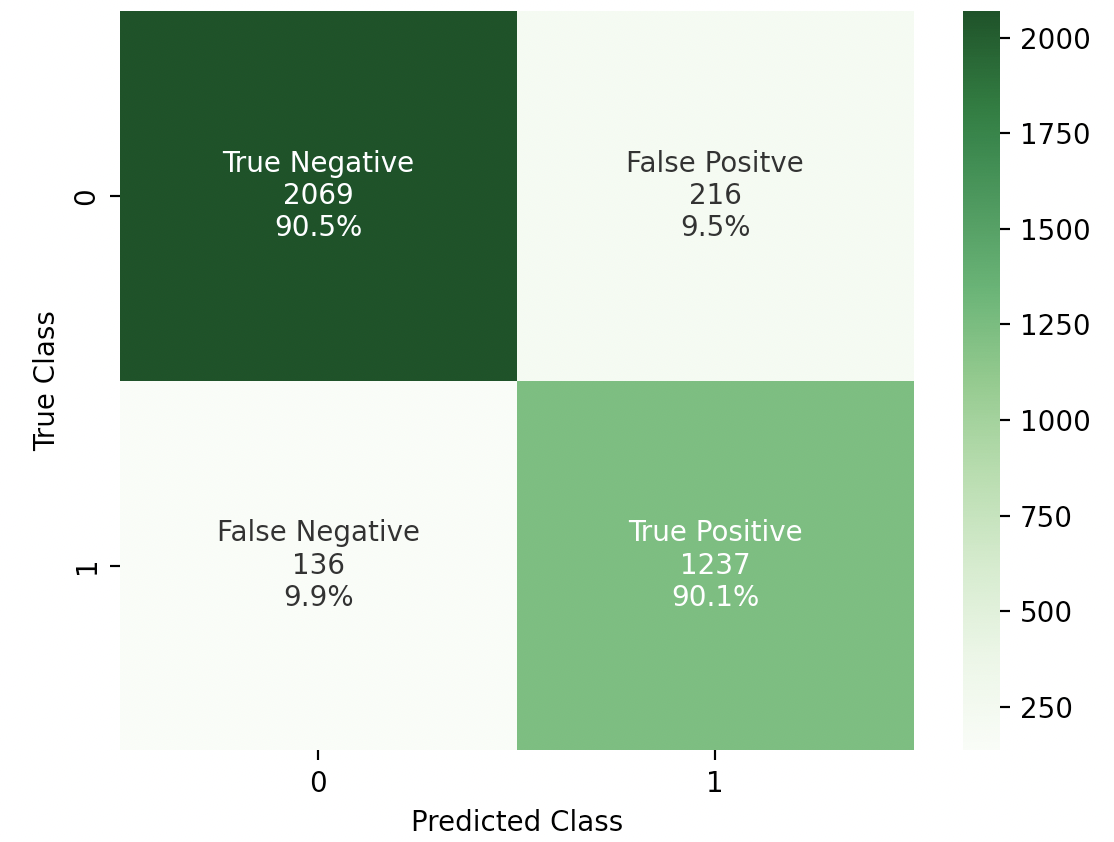
\includegraphics[width=0.78\textwidth]{images/7-results/confusion_matrix_endcap_stage_1.png}
    \caption{Confusion matrix for Stage 1 of the GNN algorithm applied to the Pixel endcap (volume 7) of the TrackML detector model.}
    \label{fig:confusion-matrix-endcap-stage-1}%
\end{figure}
  

\begin{figure}[htbp]
    \centering
    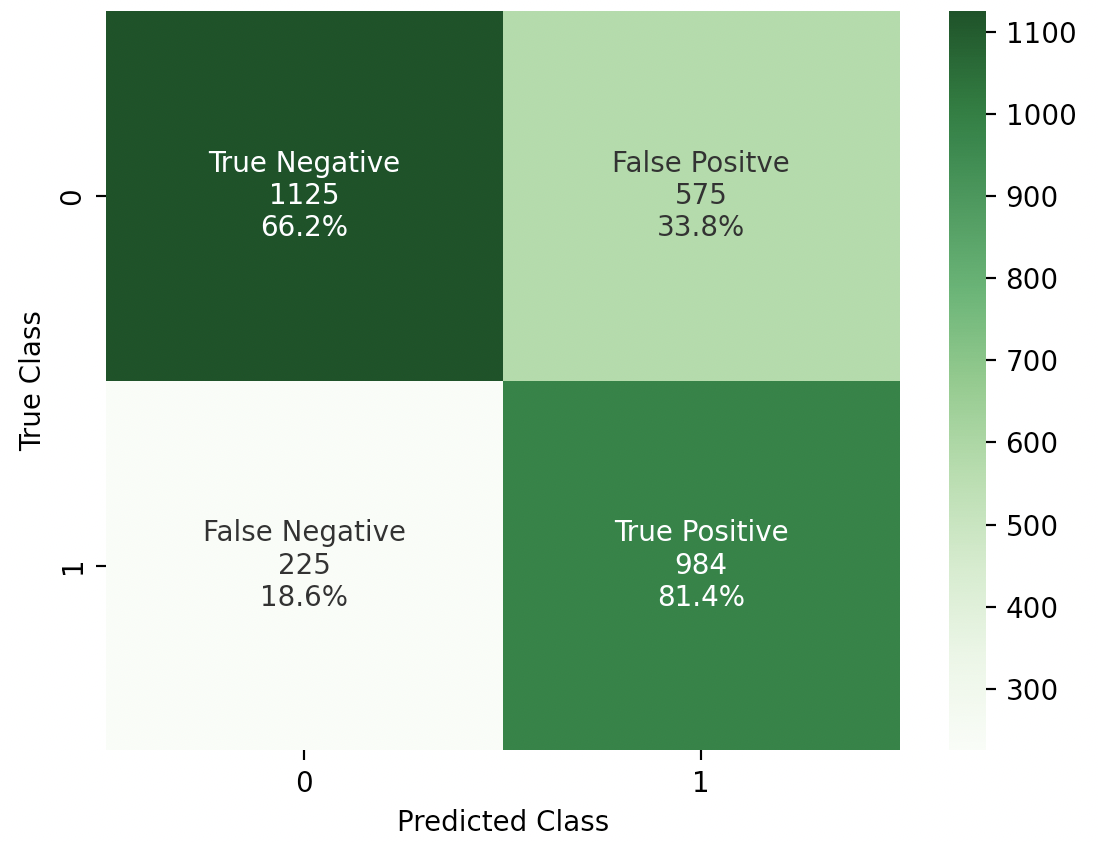
\includegraphics[width=0.78\textwidth]{images/7-results/confusion_matrix_endcap_stage_2.png}
    \caption{Confusion matrix for Stage 2 of the GNN algorithm applied to the Pixel endcap (volume 7) of the TrackML detector model.}
    \label{fig:confusion-matrix-endcap-stage-2}%
\end{figure}


For Stage 2, the TPR for identification of correct outlier edges, and hence the recall, achieved was 81.4\%, and the TNR in identification of good edges achieved was 66.2\%. With respect to MC ground truth, the precision in correct outlier edges identified during Stage 2 was found to be 63.2\%. In comparison to the prediction summary for Stage 1 shown in Figure \ref{fig:confusion-matrix-endcap-stage-1}, the second stage of the GNN algorithm does not discriminate between both classes as well as Stage 1. During Stage 2, we observe an increase in the prediction of false positives. This indicates that the algorithm begins to falsely predict a greater proportion of outlier edges, which will then affect the network connections in further algorithm stages.






\subsection{Track Reconstruction Efficiency and Purity Metrics}

The track reconstruction efficiency, $\epsilon$, provides an indication of the performance of the algorithm and is defined as the ratio of successfully reconstructed reference tracks, $n_R$, to the total number of reconstructable reference tracks, $N_R$, in a given volume of interest and is defined by Eq \eqref{eqn:reoncstruction-eff}. 


\begin{equation}
    \epsilon = \frac{n_R}{N_R}
    \label{eqn:reoncstruction-eff}
\end{equation}

Track reconstruction efficiency is calculated by first dissociating graph nodes back to hits, which means that a track candidate is now a collection of hits from several truth particles. A reconstructable reference track, $N_R$, is defined as a fully contained track within the volume of interest. As the TrackML detector can produce up to four hits per detector layer, we define a fully contained track to have at least twelve hits within the region of interest. Particles with twelve or more hits and proposed tracks with twelve or more hits are considered. Successfully reconstructed reference tracks, $n_R$, are defined as having at least 50\% of its hits from the same truth particle, $N_{hits}$. If $N_{hits} \geq 0.5 \times N_{ref}$, where $N_{ref}$ is the number of reference hits in the volume of interest, then the truth particle reference track is considered as reconstructed.

Initially, all reference tracks with $p_{\text{T}} \ge$ 150 MeV are selected and the efficiency is calculated for this. The cut in then increased to select reference tracks with $p_{\text{T}} \ge$ 1 GeV. Table \ref{tab:trackml-track-recon-effs} summarises the track reconstruction efficiencies obtained for fully contained MC truth tracks within volume 7 of the TrackML Pixel detector.


\begin{table}[htbp]
\caption{Summary of track reconstruction efficiencies obtained for fully contained MC truth tracks within volume 7 of the TrackML Pixel detector, which have been extracted using the GNN iterative algorithm developed. $n_R$ is the number of successfully reconstructed reference tracks, $N_R$ is the total number of reconstructable reference tracks and $\epsilon$ is the track reconstruction efficiency. }

\begin{center}
\begin{tabular}{cccc}
\toprule
Threshold & $n_R$ & $N_R$ & $\epsilon$ \\
\hline
$p_{\text{T}} \ge$ 150 MeV    & 1167  & 1347  &  86.6\%    \\
$p_{\text{T}} \ge$ 1 GeV      & 180   & 192   &  93.8\%    \\
\bottomrule
\end{tabular}
\end{center}
\label{tab:trackml-track-recon-effs}
\end{table}

%For fully contained MC truth tracks within volume 7 of the TrackML Pixel detector with $p_{\text{T}} \geq$ 150MeV, the track reconstruction efficiency obtained was 86.2\%, where $n_R = 614$ and $N_R = 712$. Similarly, for fully contained MC truth tracks within volume 7 of the TrackML Pixel detector with $p_{\text{T}} \geq$ 1GeV the track reconstruction efficiency obtained was 93.8\%, where $n_R = 180$ and $N_R = 192$.

% correct data - checked
% pt cut of 150 MeV
% Total num of reconstructed tracks: 1167
% Total num of reference tracks: 1347
% Track reconstruction efficiency:  86.637 %

% pt cut of 1 GeV
% Total num of reconstructed tracks: 180
% Total num of reference tracks: 192
% Track reconstruction efficiency:  93.750 %


Each track is matched with the ground truth majority particle sharing with it the greatest hit number, $N_{truth}$. The ratio of $N_{truth}$ to the number of hits for the reconstructed track, $N_{hits}$, defines the track purity, whilst the ratio of $N_{truth}$ to the number of hits of the underlying particle, $N_{phits}$, defines the particle purity. Both the track purity and particle purity must be greater than 50\%. This criteria coincides with the definition of an accepted track candidate stated in the TrackML competition \cite{kaggle-trackml}.

The purity distributions are shown in Figure \ref{fig:trackml-results-endcap-purity}. The average track purity and particle purity achieved for all extracted candidates in volume 7 after application of the GNN algorithm was 99.0\% for both quantities. There is a small tail in the distribution, however this is negligible as it is several orders of magnitude lower than the main peak. Both purity distributions indicate that the application of the OU process within the KF for track extraction works well to model the influence of the magnetic field for the given $p_{\text{T}}$ range.

\begin{figure}[htbp]
    \centering
    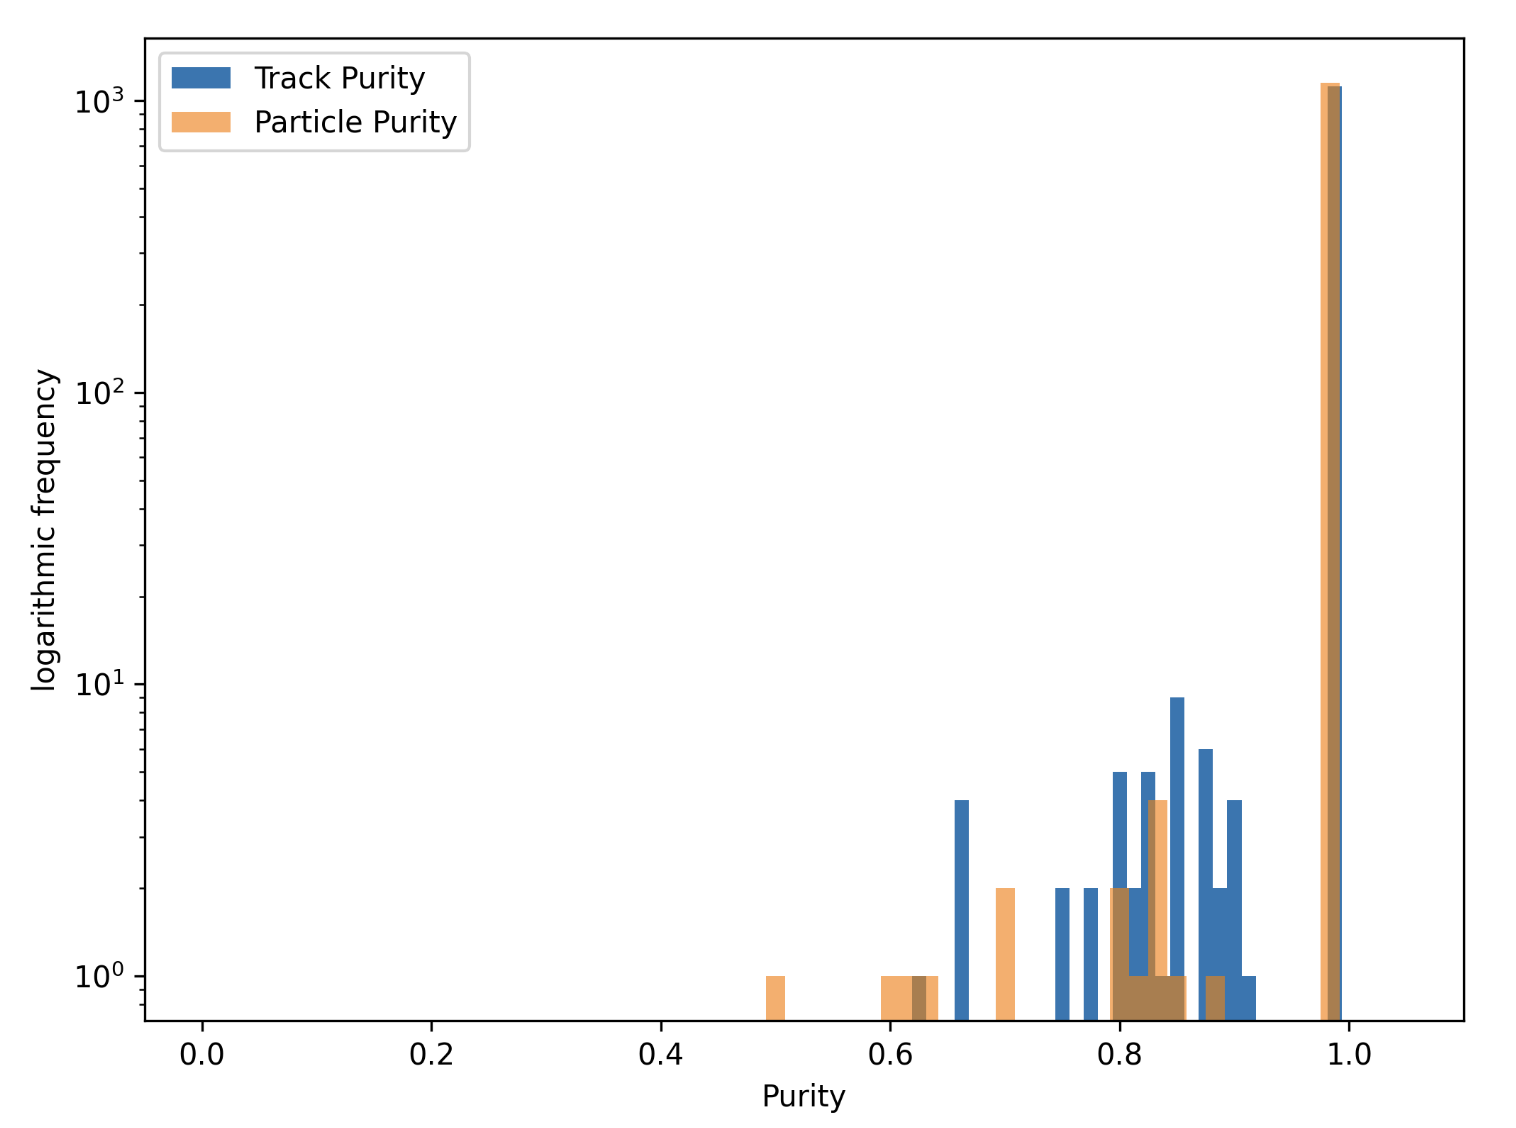
\includegraphics[width=0.75\textwidth]{images/7-results/endcap-purity-log.png}
    \caption{Purity distributions for extracted track candidates after application of the GNN algorithm for track reconstruction within volume 7 of the TrackML Pixel detector with $p_{\text{T}} \geq$ 150MeV.}
    \label{fig:trackml-results-endcap-purity}%
\end{figure}


%present the average over many events here
Executing the GNN algorithm on 50 simulated TrackML events, the average track reconstruction efficiency achieved for fully contained tracks within volume 7 and with $p_{\text{T}} \geq$ 1GeV was 93.3\%. The average track purity and average particle purity achieved were 99.0\% for both quantities.



%\subsection{Performance Evaluation on Volumes 7 and 9}





\subsection{Execution Times}

The GNN algorithm was executed on a MacOS machine, M1 Pro chip, 16GB RAM, with no multi-threaded functions. The minimum execution time for the GNN algorithm to process 1 simulated event in volume 7 of the TrackML detector was 45.6s. Table \ref{tab:trackml-endcap-execution-times} and Figure \ref{fig:execution-time-endcap-1} show the breakdown of execution time for each stage of the GNN algorithm. The initialization of the graph network adopts the majority of the execution time, where the remaining algorithmic components comprise 15.9s in execution time. Graph network initialization comprises of a conversion of TrackML hit data to nodes and edges, as well as construction of track state estimates $X_{ij}$ and covariances $C_{ij}$. Reading and writing into the graph network implemented using the NetworkX library contributes a significant proportion of execution time. Whereas, the execution time for each stage of the GNN algorithm, as well as track extraction, is notably small.

\begin{table}[htbp]
\caption{Breakdown of execution time and cumulative execution time for each stage of the GNN algorithm applied to volume 7 of the TrackML detector.}
\begin{center}
\begin{tabular}{lccc}
\toprule
GNN Algorithm Stage & Time (s) & Cumulative Time (s) & \% \\
\hline
Graph Network Initialization    & 29.7  & 29.7  &  65.1    \\
Stage 1: GMR                    & 3.5   & 33.2   &  7.7    \\
Track Extraction 1              & 4.8   & 38.0   &  10.5    \\
Stage 2: Information Aggregation & 3.2   & 41.2   &  7.0    \\
Track Extraction 2              & 4.4   & 45.6   &  9.6    \\
\bottomrule
\end{tabular}
\end{center}
\label{tab:trackml-endcap-execution-times}
\end{table}

\begin{figure}[htbp]
    \centering
    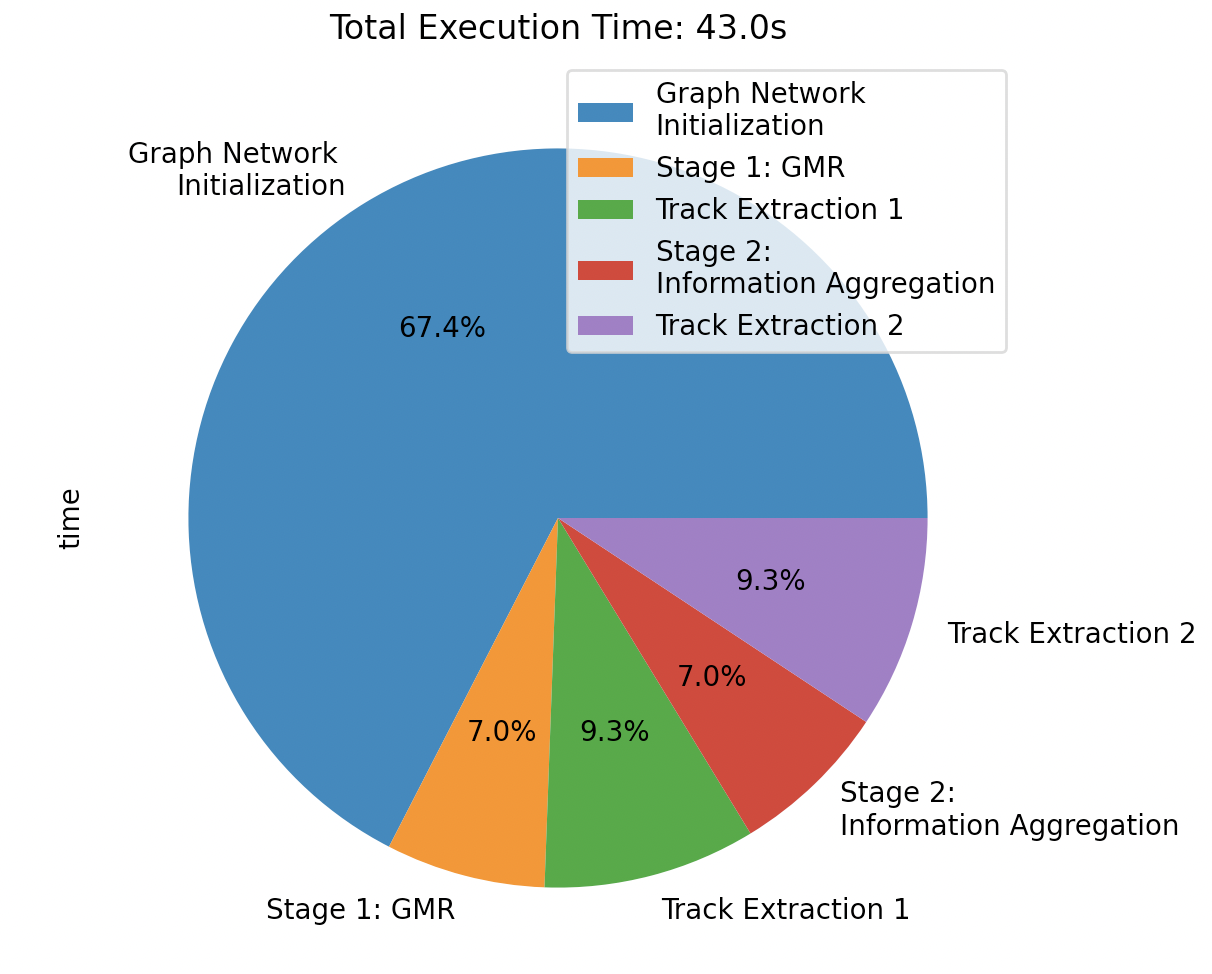
\includegraphics[width=0.7\textwidth]{images/7-results/execution-time-endcap-1.png}
    \caption{Breakdown of execution time for each stage of the GNN algorithm applied to volume 7 of the TrackML detector.}
    \label{fig:execution-time-endcap-1}%
\end{figure}






\subsection{Advantages of the KF Implementation}

An important feature of the KF application is that reconstruction of curved tracks is possible using a low-dimensionality model. By assuming a slow change in track direction, a dynamic model for the KF is constructed using the OU process. The OU process implicitly takes into account the track curvature, without the need to extend the track state to contain additional parameters.







\section{Extension to the Pixel Barrel Region}
\label{chapter-7-outlook}


The application of the GNN algorithm is extended to the Pixel barrel region and the right endcap of the TrackML detector, in order to cover the entire Pixel detector volumes $\{7, 8, 9\}$, with reference to Figure \ref{fig:trackml-detector-image}. The graph network is constructed using 38,365 nodes contained within these volumes from a simulated TrackML event, and 201,748 predicted edges are formed using the FASTrack algorithm \cite{Dmitry-fasttrack-addtest}. For this particular test the same initial $p_{\text{T}}$ cut as executed in Section \ref{performance-eval-endcap-vol-7-start} was used for graph segment generation: $p_{\text{T}} \ge 150$ MeV. Figure \ref{fig:trackml-results-barrel-endcap} illustrates the extracted track candidates after application of the GNN algorithm. 

It is clear to see from Figure \ref{fig:trackml-results-barrel-endcap-extracted-xy} that track candidates are extracted uniformly across all $ 0^{\circ} \leq \phi \leq 360^{\circ}$ during Stages 1 and 2 of the GNN algorithm. This is as expected due to the rotational symmetry of the detector in the transverse plane. 

Figure \ref{fig:trackml-results-barrel-endcap-extracted-rz} shows the extracted track candidates viewed from the $r$-$z$ plane, where the algorithm works effectively in both the left and right Pixel endcap regions, however the proportion of track candidates extracted in the Pixel barrel is significantly less. During the Stage 1, a total of 1629 track candidates were successfully extracted. During Stage 2 a further 294 track candidates were extracted and in Stage 3 a further 7 were extracted.

In Stage 1, we observe track candidates extracted uniformly in both endcaps. This is primarily due to the parallel geometry of detector layers and telescopic trajectory of the corresponding tracks, hence there are far fewer ambiguities to resolve in comparison to the barrel region. In contrast to this, during Stage 2 we observe the majority of track candidates extracted are located at a larger $\theta$ to the $z$-axis (smaller $\eta$) in comparison to Stage 1. This is the transition region between the barrel and endcap layers. We also observe a small proportion of track candidates extracted which are contained only within the barrel region.


\begin{figure}[htbp]%
    \centering
    \subfloat[\centering $x$-$y$ plane view]{{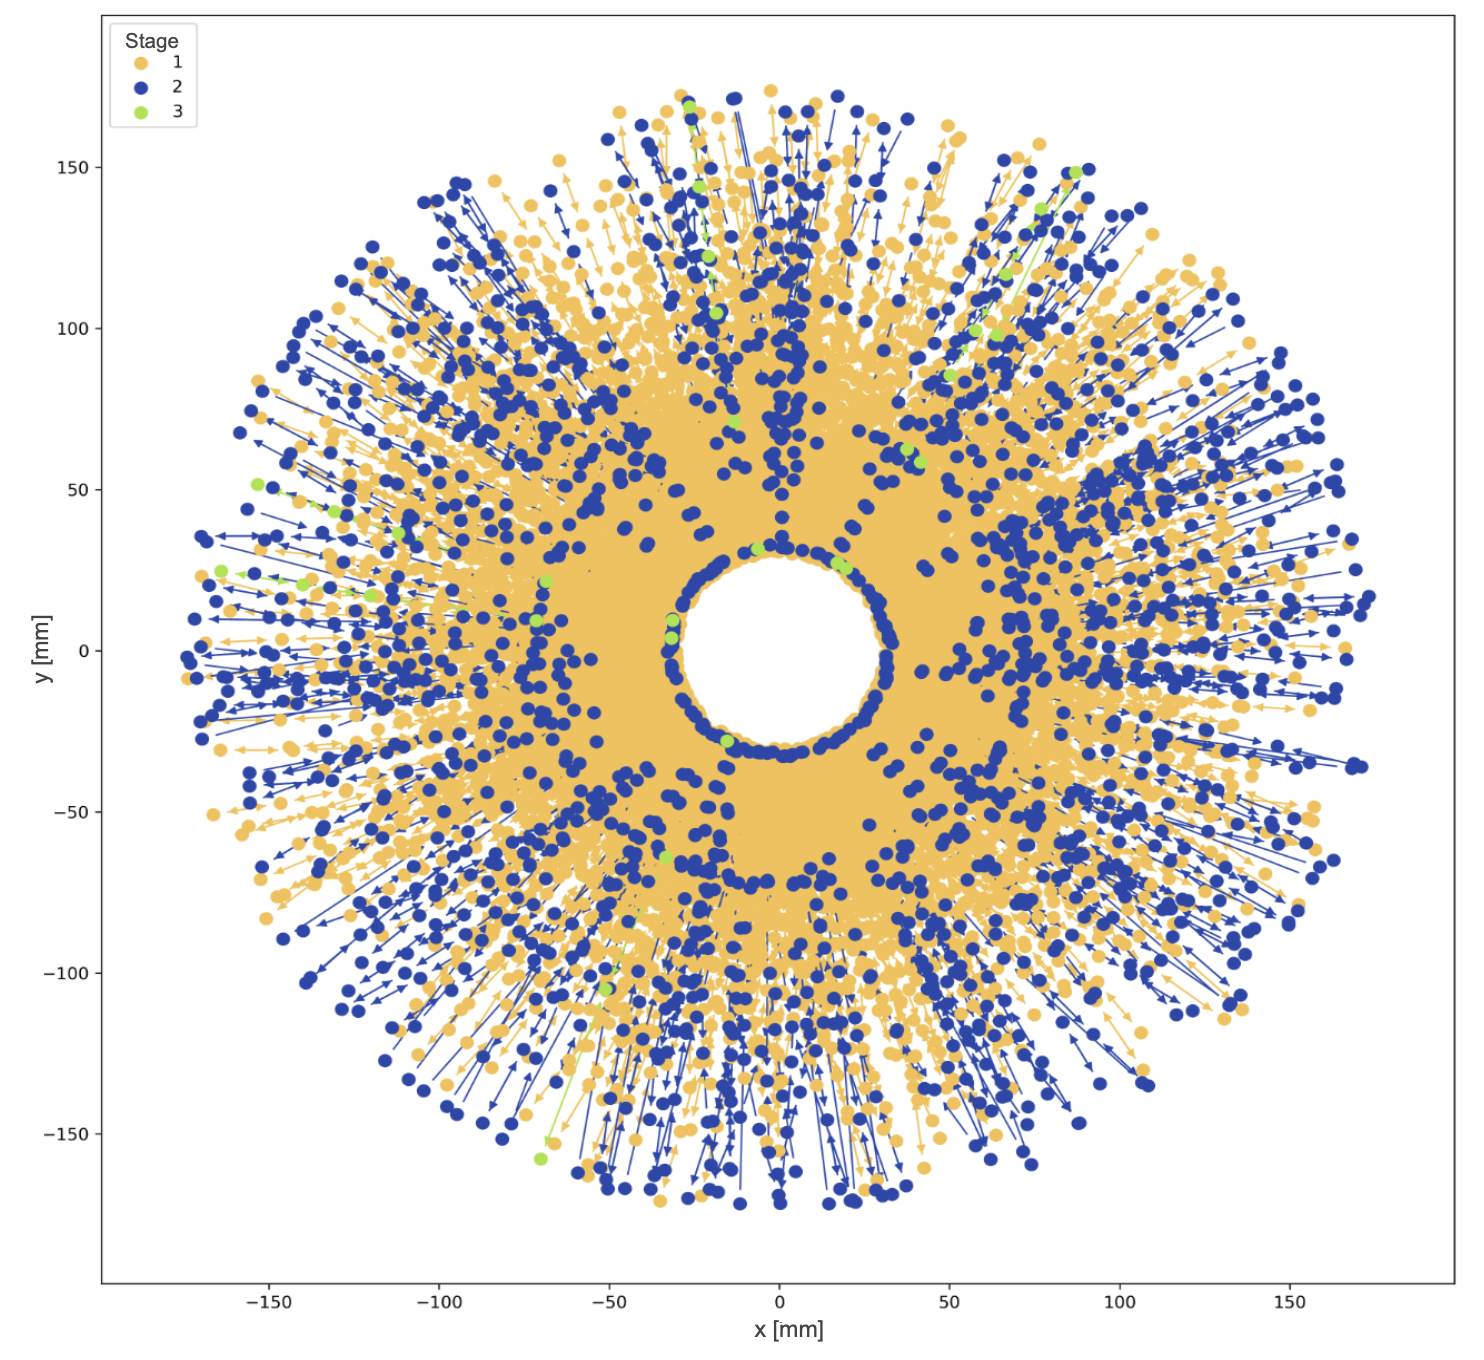
\includegraphics[width=10cm]{images/7-results/trackml-endcap-barrel-extracted-xy.png} } \label{fig:trackml-results-barrel-endcap-extracted-xy}}%
    \hfill
    %\qquad
    \subfloat[\centering $r$-$z$ plane view]{{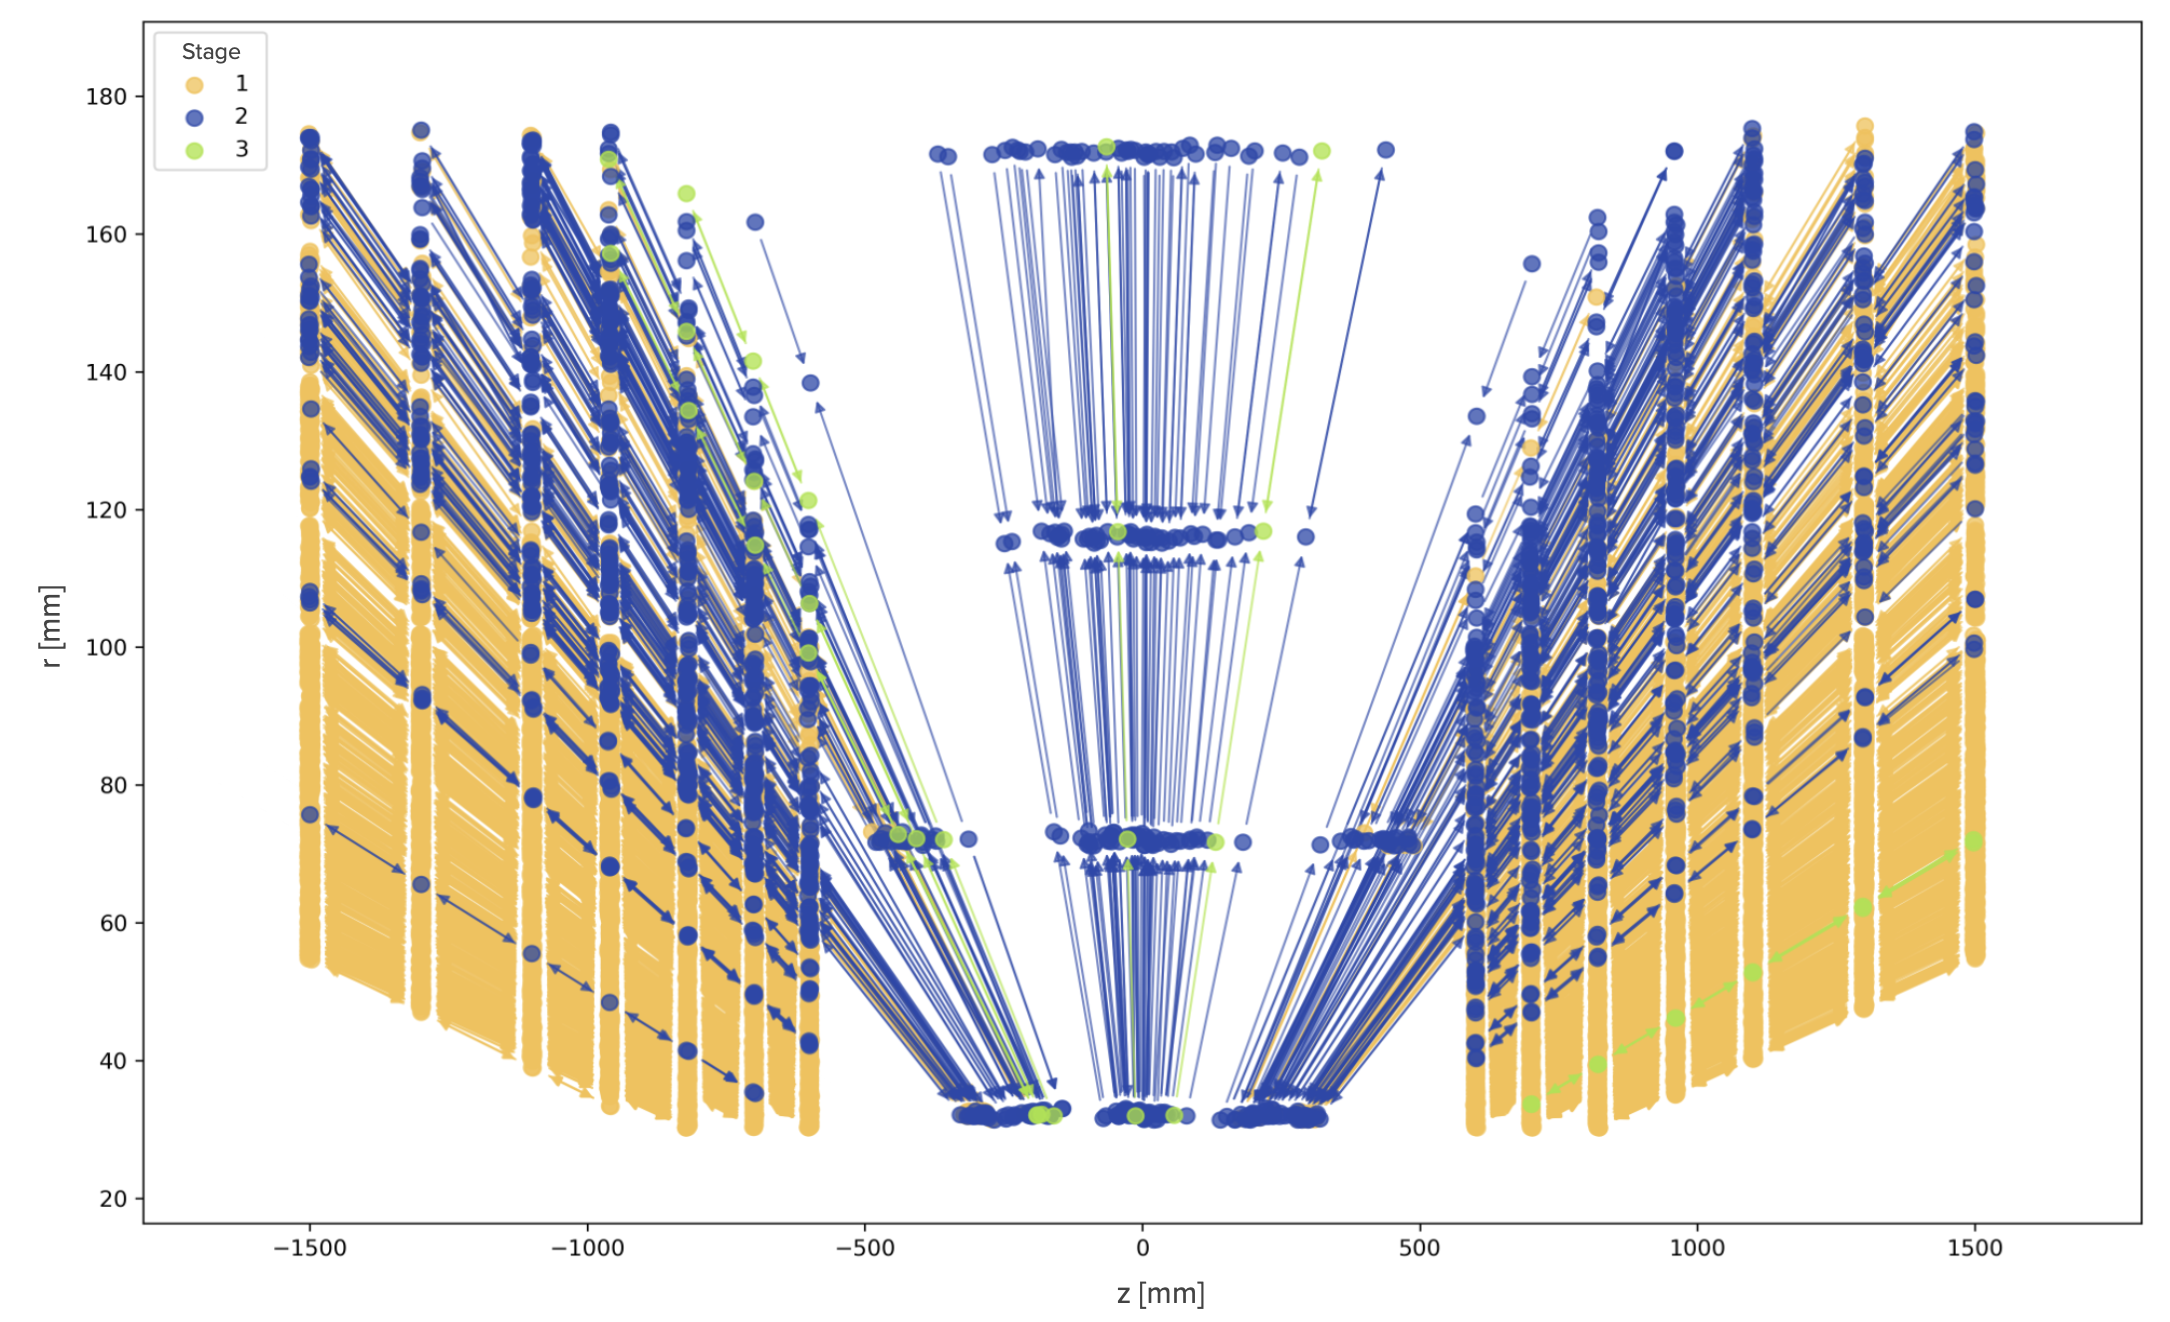
\includegraphics[width=14.5cm]{images/7-results/trackml-endcap-barrel-extracted-rz.png} } \label{fig:trackml-results-barrel-endcap-extracted-rz}}%
    \caption{Extracted track candidates post application of the iterative GNN algorithm onto the Pixel detector of the TrackML model. Track candidates are iteratively extracted after each stage of the GNN algorithm, shown by the legend.}%
    \label{fig:trackml-results-barrel-endcap}%
\end{figure}






\subsection{Confusion Matrices}

The following confusion matrices depict the prediction summary of the GNN algorithm onto the TrackML simulated event, where predicted class 1 indicates the prediction of outlier edges with respect to MC truth and predicted class 0 indicates the prediction of good edges to remain active in the network. The confusion matrix for Stage 1 of the GNN algorithm applied to the Pixel barrel and endcap regions is shown in Figure \ref{fig:confusion-matrix-barrel-endcap-stage-1}.


The TPR for identification of correct outlier edges achieved was 92.3\%, and the True Negative Rate (TNR) in identification of good edges achieved was 84.9\%. With respect to MC ground truth, the proportion of correct outlier edges identified during Stage 1 of the GNN algorithm, and hence the precision, was found to be 95.6\%. The recall in correct outlier edges identified during Stage 1 was 92.3\%. Similar to Section \ref{confusion-matrices-endcap-trackml} these results indicate that the GMR technique of the GNN-algorithm works well for resolving ambiguities in the graph network.

\begin{figure}[htbp]
    \centering
    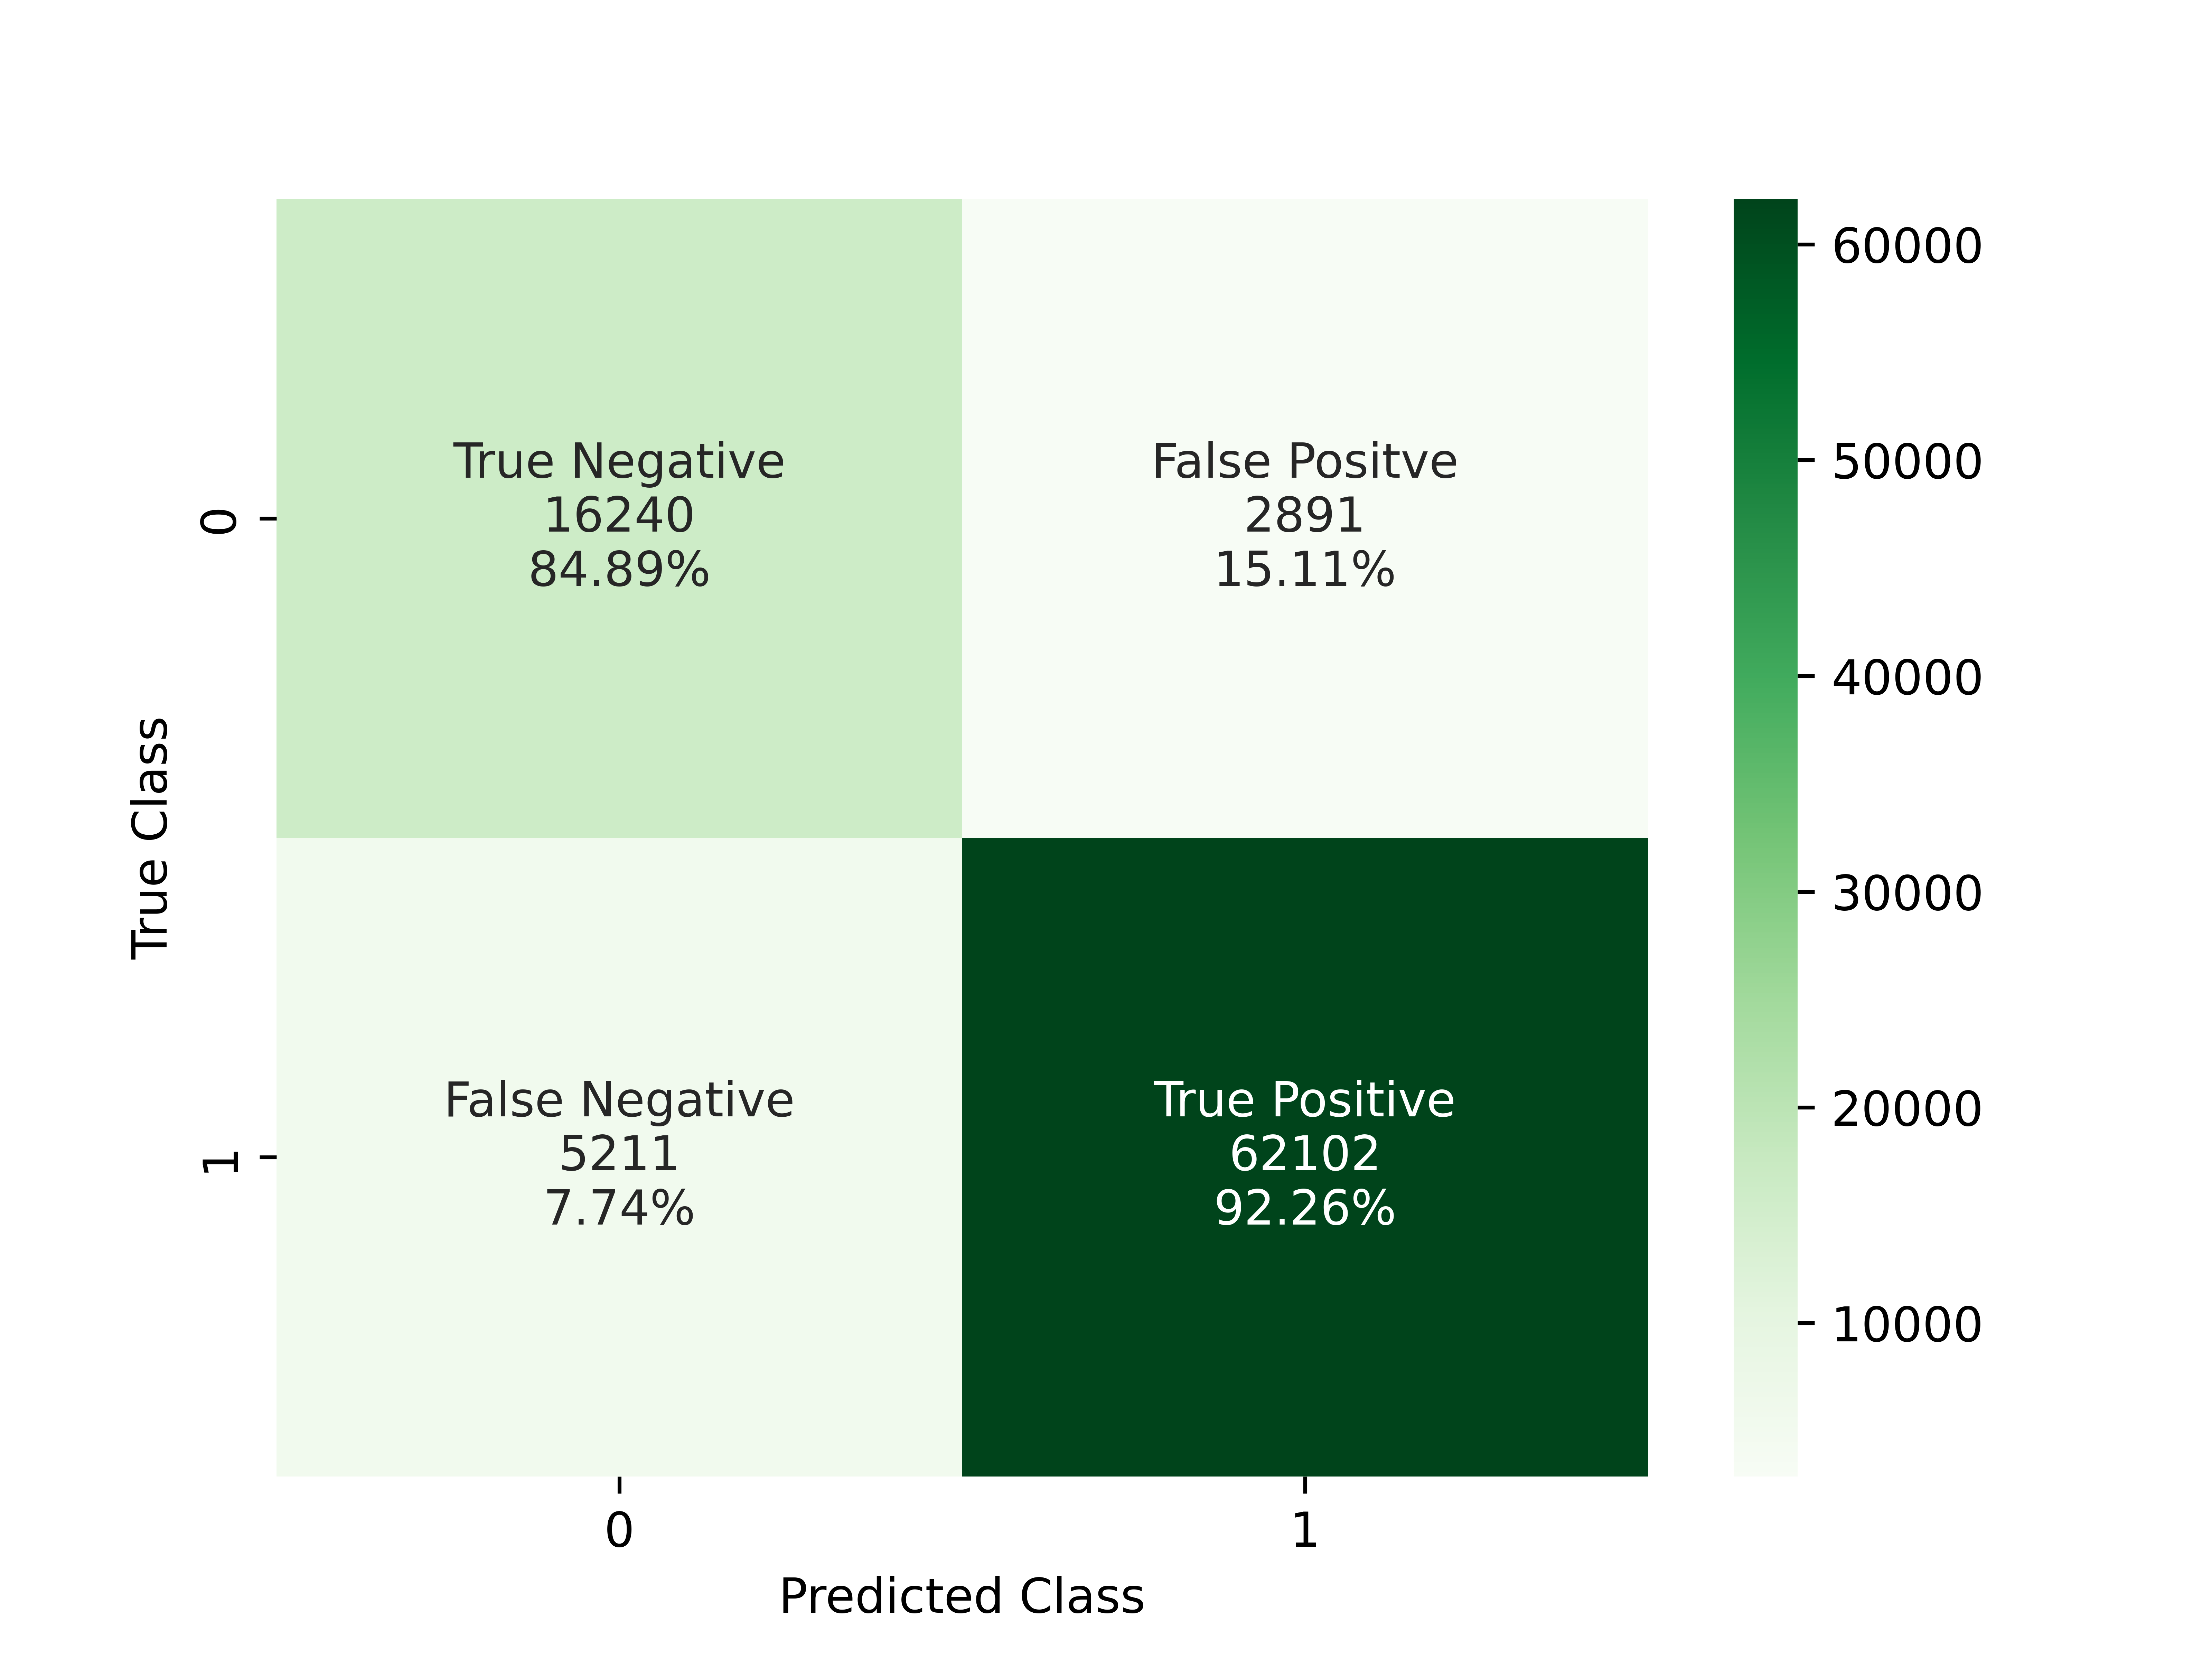
\includegraphics[width=0.79\textwidth]{images/7-results/confusion_matrix_barrel_stage_1.png}
    \caption{Confusion matrix for Stage 1 of the GNN algorithm applied to the Pixel barrel and endcap of the TrackML detector model.}
    \label{fig:confusion-matrix-barrel-endcap-stage-1}%
\end{figure}

The confusion matrix for Stage 2 of the GNN algorithm applied to the Pixel barrel and endcap regions is shown in Figure \ref{fig:confusion-matrix-barrel-endcap-stage-2}.


\begin{figure}[htbp]
    \centering
    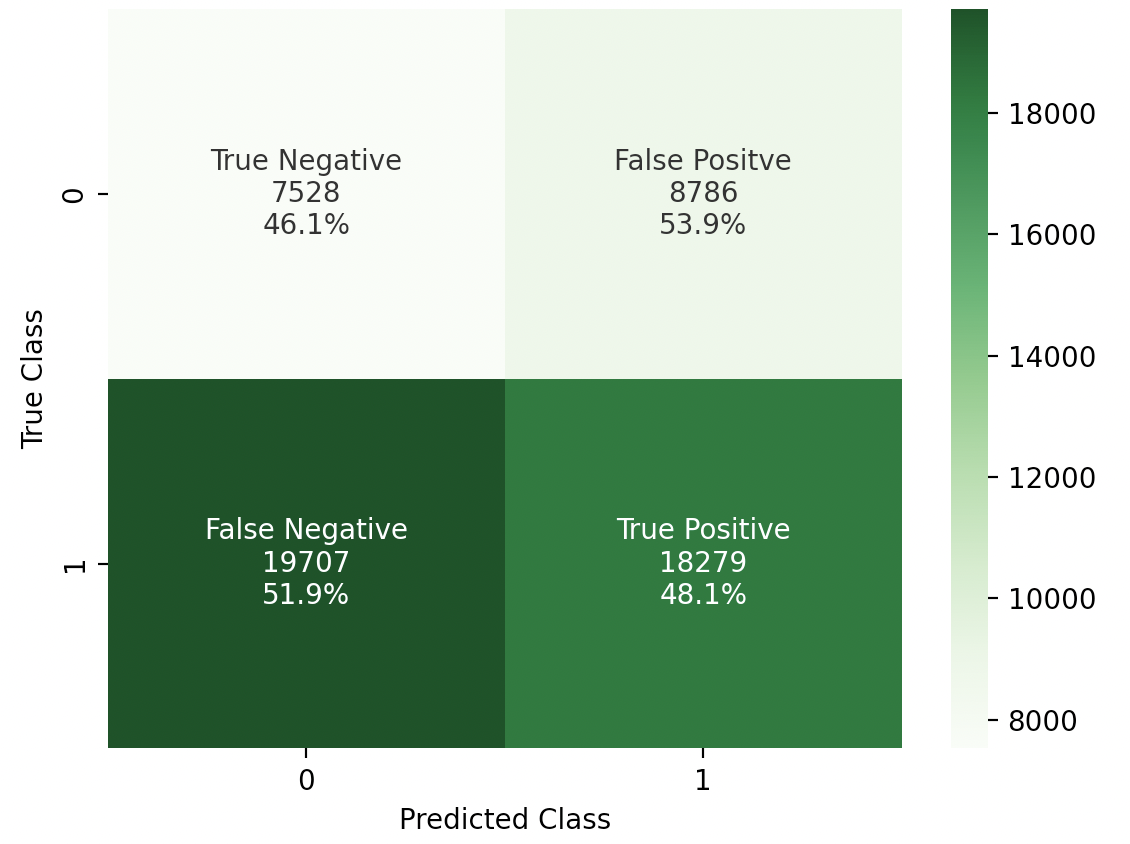
\includegraphics[width=0.79\textwidth]{images/7-results/confusion_matrix_barrel_stage_2.png}
    \caption{Confusion matrix for Stage 1 of the GNN algorithm applied to the Pixel barrel and endcap of the TrackML detector model.}
    \label{fig:confusion-matrix-barrel-endcap-stage-2}%
\end{figure}

For Stage 2, the TPR for identification of correct outlier edges, and hence the recall, achieved was 48.1\%, and the TNR in identification of good edges achieved was 46.1\%. With respect to MC ground truth, the precision in correct outlier edges identified during Stage 2 was found to be 67.5\%. In comparison to the prediction summary for Stage 1 shown in Figure \ref{fig:confusion-matrix-barrel-endcap-stage-1}, the second stage of the GNN algorithm does not discriminate between both classes as well as Stage 1, as there is a much greater proportion of false positives and false negatives. This suggests that the algorithm begins to falsely predict a greater proportion of outlier edges, which will then affect the network connections in further algorithm stages.




%\subsection{Track Reconstruction Efficiency and Purity Metrics}


% \begin{figure}[htbp]
%     \centering
%     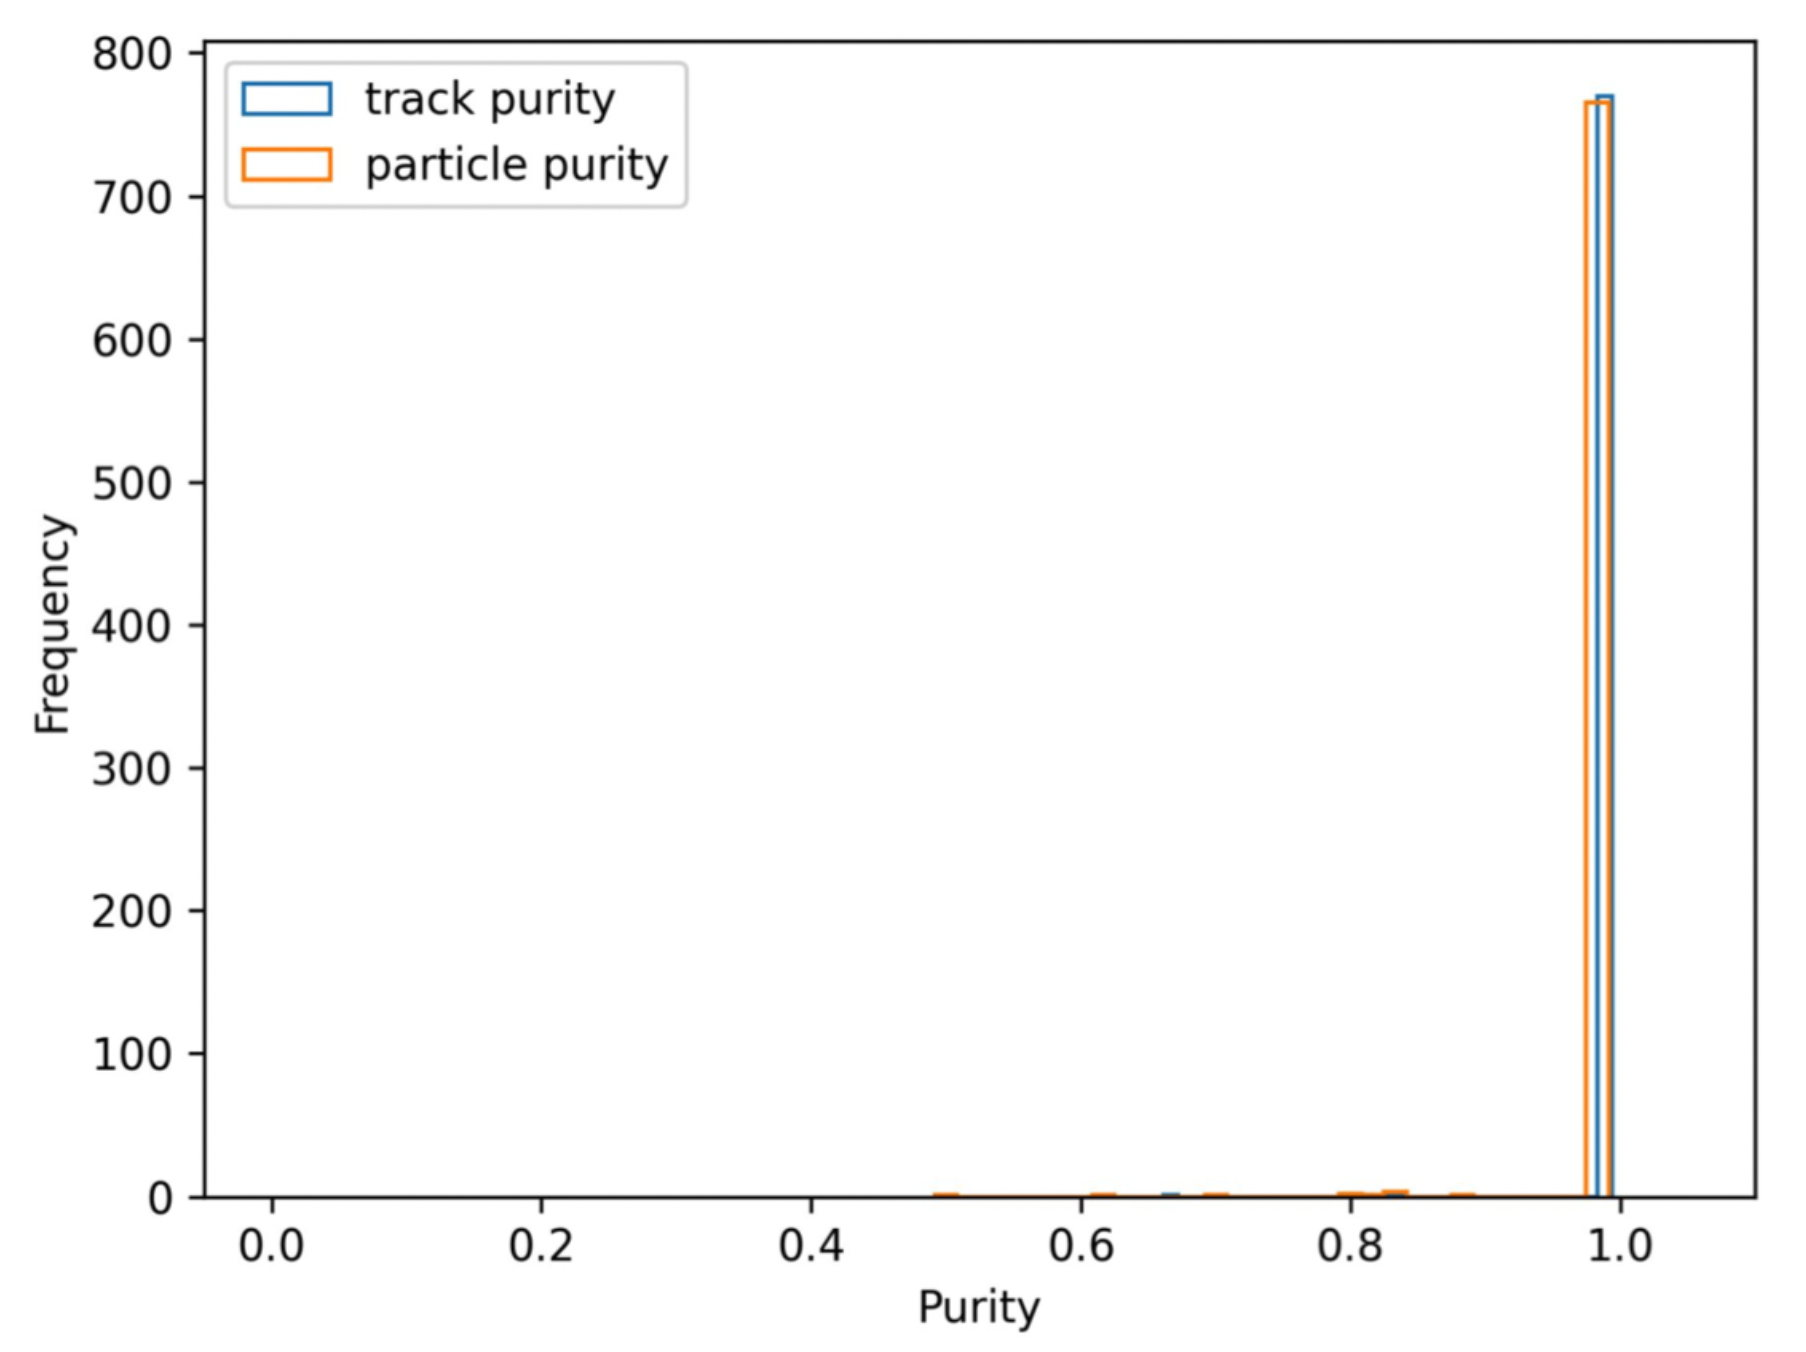
\includegraphics[width=0.7\textwidth]{images/7-results/endcap-purity.png}
%     \caption{Purity distributions for application of the GNN algorithm for track reconstruction on the Pixel barrel and endcap regions of the TrackML detector}
%     \label{fig:trackml-results-endcap-barrel-nodes-purity}%
% \end{figure}


% \subsection{Execution Times}



% \subsection{Remaining Network Post Track Extraction}

% The node density in the barrel is ... times greater compared to the endcap regions, and the edge density is .... which is a contributing factor towards this.

% \begin{figure}[htbp]
%     \centering
%     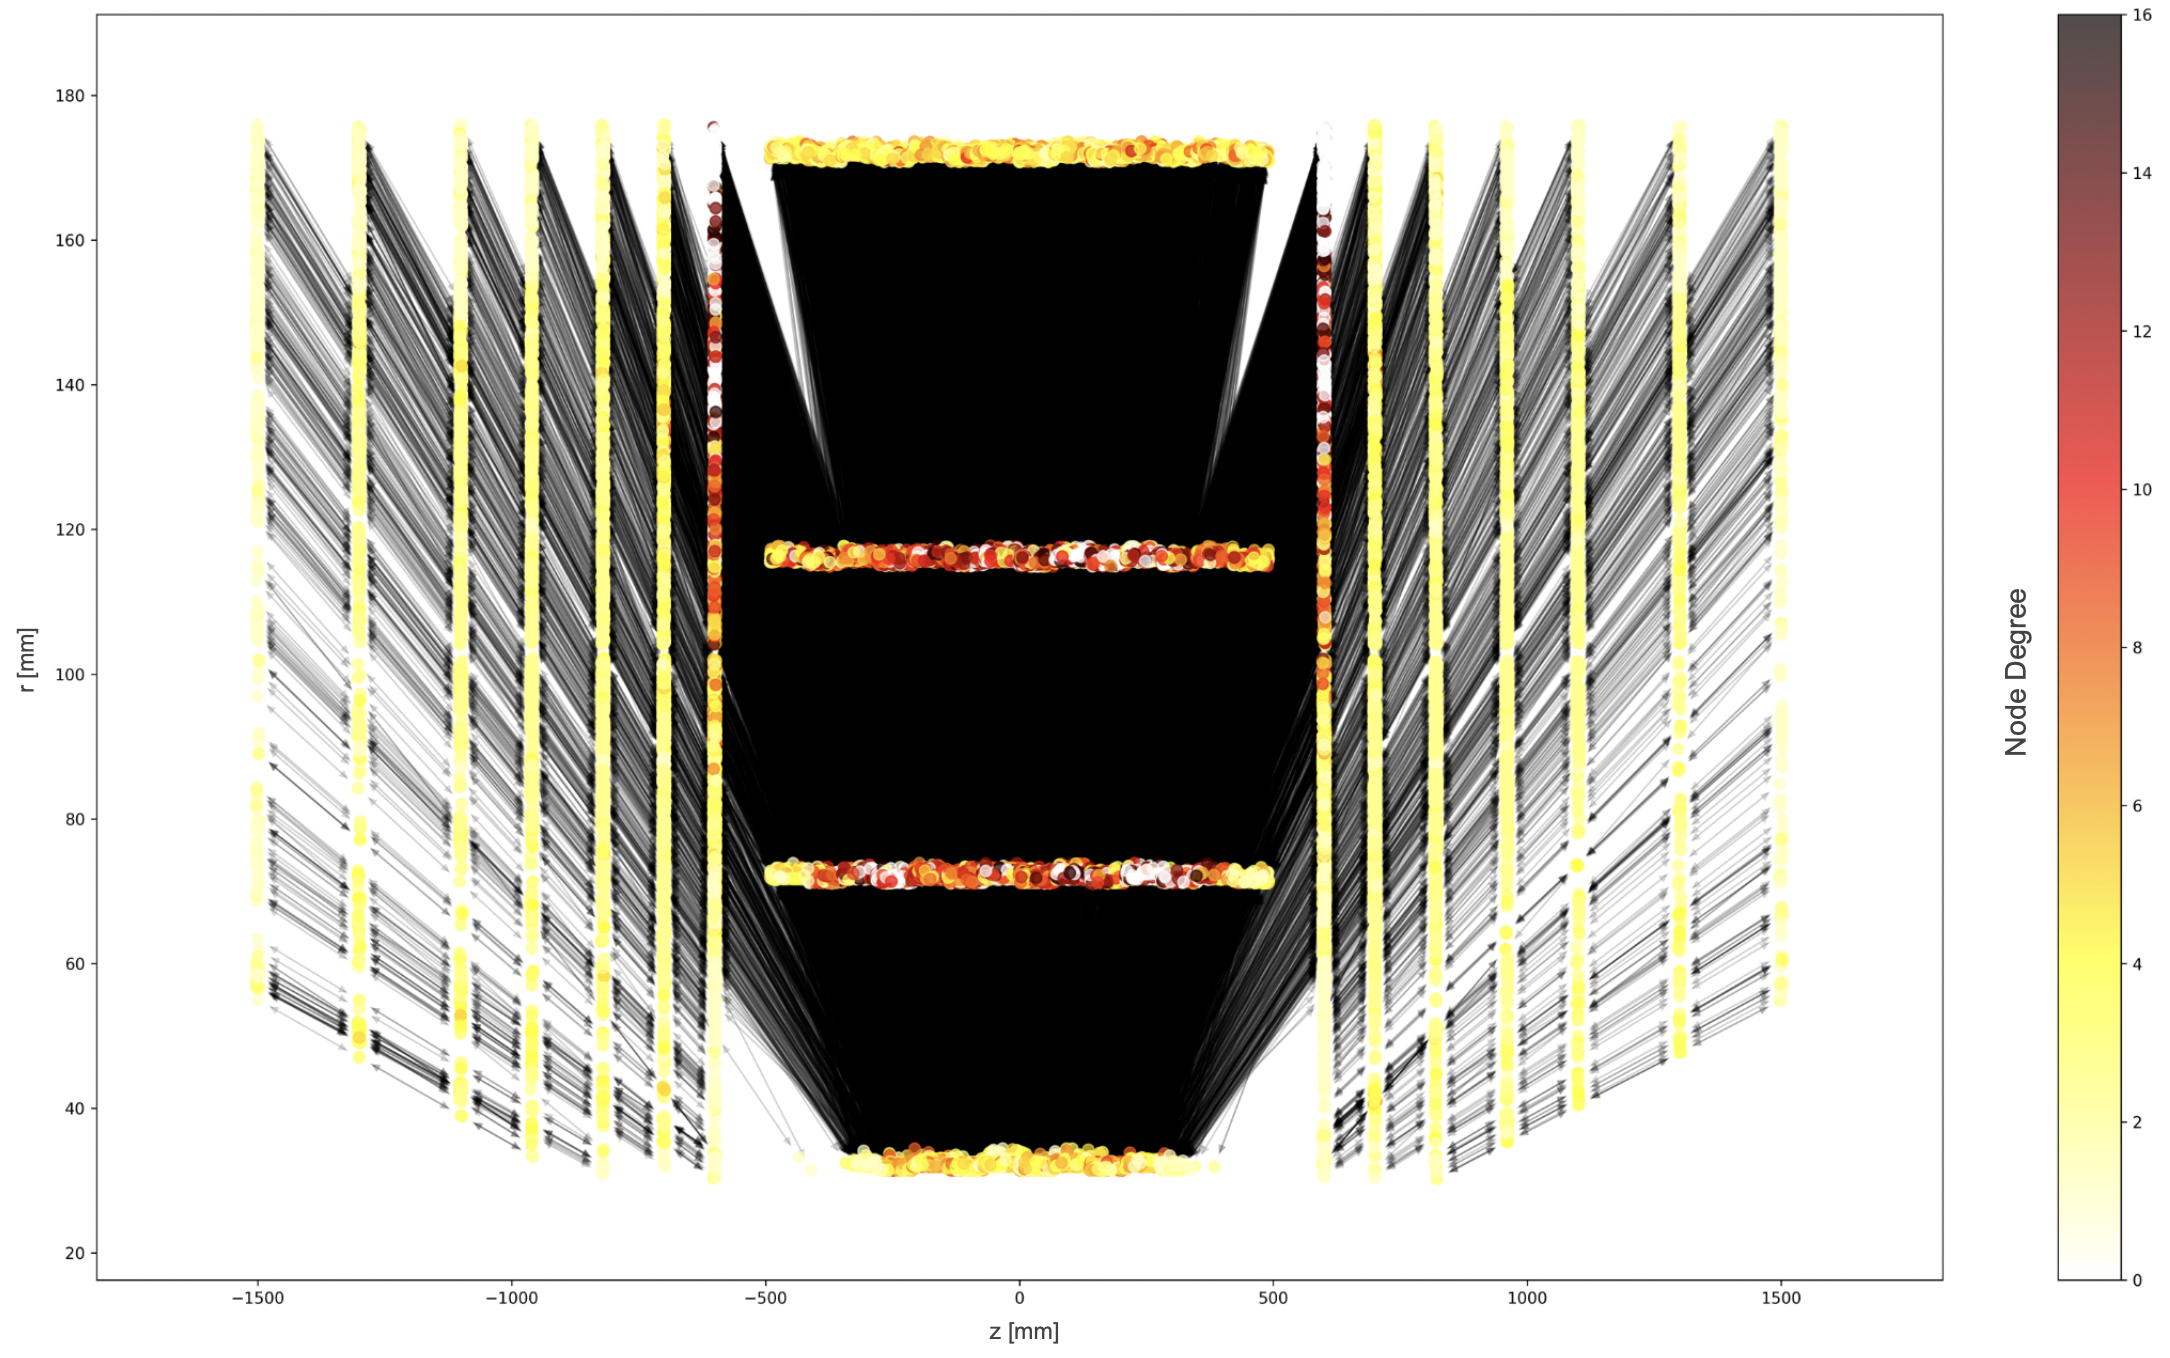
\includegraphics[width=0.99\textwidth]{images/7-results/trackml-barrel-remaining-node-degree.png}
%     \caption{TODO: regenerate this plot but with the node degree inverted!!! }
%     \label{fig:trackml-results-barrel-endcap-remaining-node-degree}%
% \end{figure}







\section{Improvements and Other Approaches}



\subsection{Improvement for Extrapolation in r-z Plane}

In general, a track state in $r$-$z$ plane is defined as a track position at some reference surface (constant radius $r$ or constant $z$ position) and the inverse track inclination angle as outlined in Section \ref{chapter-6-end-of-derivation}. Due to the orientation of the detector layers, the extrapolation can result in a change of reference surface type. One such example is an extrapolation from the Pixel barrel layer at constant $r$ to Pixel endcap layer at constant $z$. Naturally, there are four possible cases for extrapolation; barrel-to-barrel, barrel-to-endcap, endcap-to-barrel and endcap-to-endcap, and each case should be considered individually. Figure \ref{fig:improvement-extrapolation} shows an illustration of the extrapolation from a barrel to endcap layer.


\begin{figure}[htbp]
    \centering
    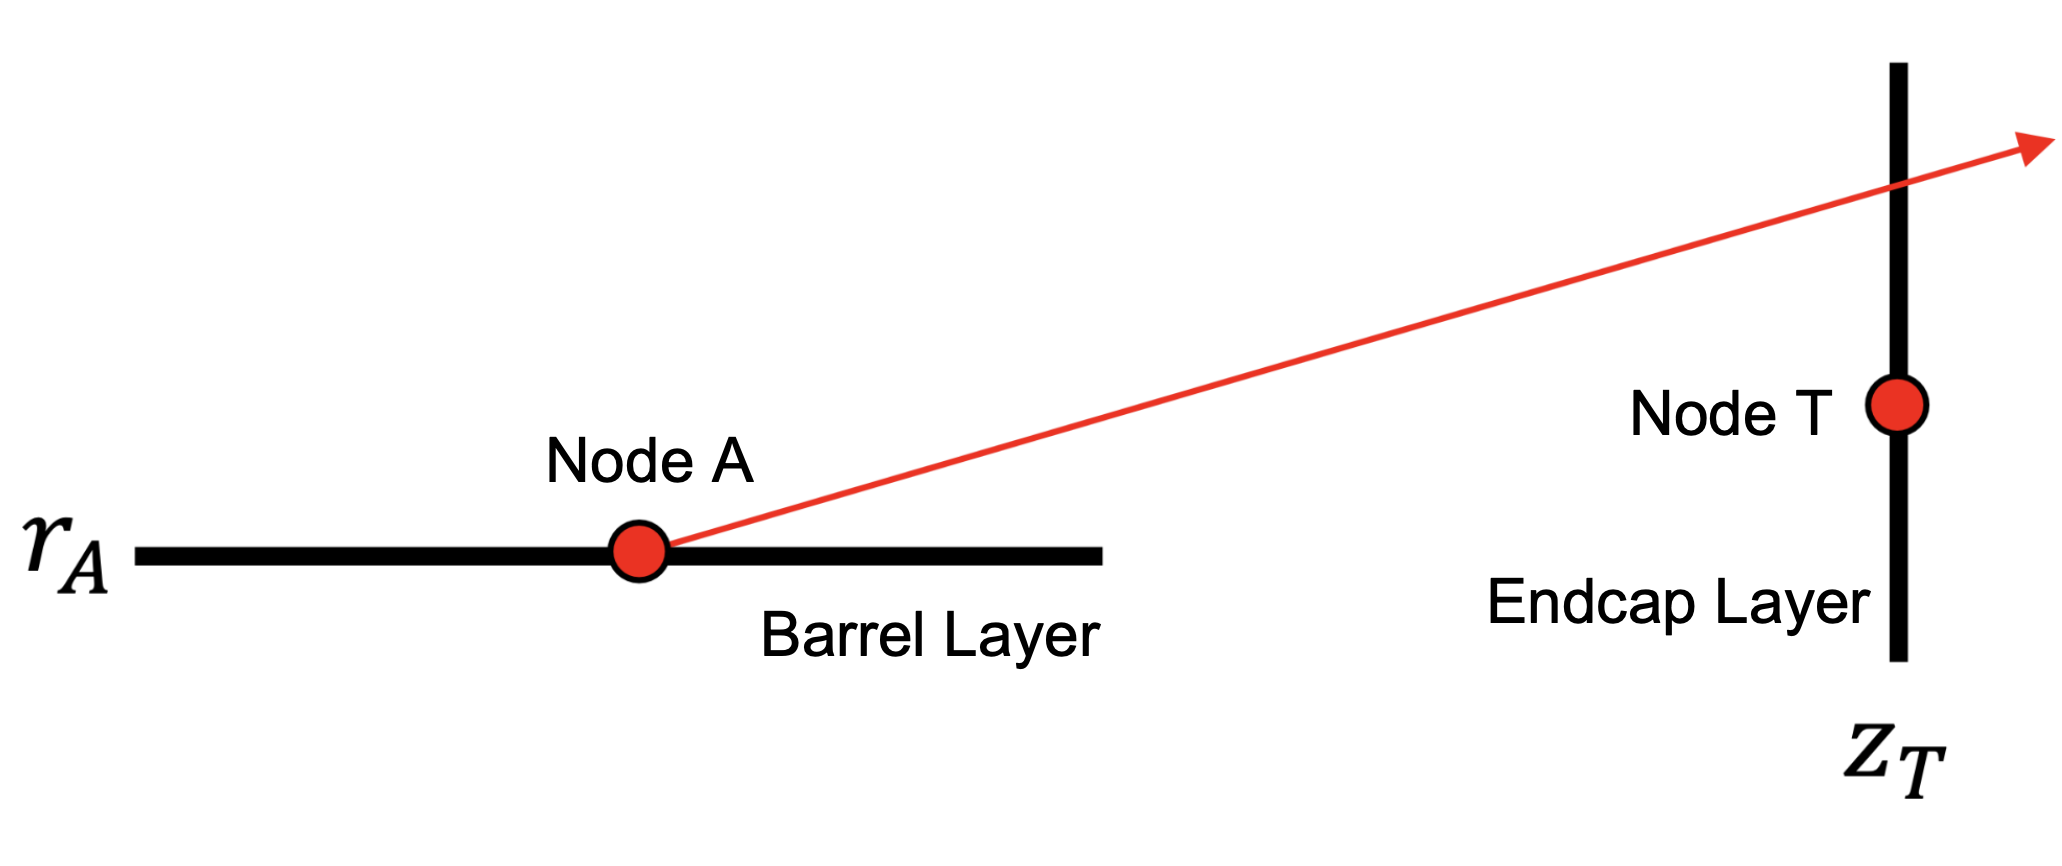
\includegraphics[width=0.8\textwidth]{images/7-results/improvement-extrapolation.png}
    \caption{Illustration of track state extrapolation from node A located in a barrel layer at constant radius $r$, to the target node, node T located in an endcap layer at constant $z$-position.}
    \label{fig:improvement-extrapolation}%
\end{figure}


The initial track state is at node A with its $z$-position and some estimate of inverse track inclination $\tau_A$. The final track state is at a target node T with its $z$-position and consists of an extrapolated $r$-position and $\tau_T$. This is described by Equations \eqref{eqn:extrapolation-improvement-1}  and \eqref{eqn:extrapolation-improvement-2}, and hence this model would lead to a different form of the extrapolation Jacobian.

\begin{equation}
    \begin{bmatrix} z_A \\ \tau_A \end{bmatrix} 
    \rightarrow
    \begin{bmatrix} r_T \\ \tau_T \end{bmatrix} 
    \label{eqn:extrapolation-improvement-1}
\end{equation}

\begin{equation}
    r_T = r_A + \frac{z_T - z_A}{\tau_A}, \quad \tau_T = \tau_A
    \label{eqn:extrapolation-improvement-2}
\end{equation}


Exploring this general case of extrapolation in the $r$-$z$ plane is one such enhancement for the implementation of the KF and may provide an improvement in the precision of track state estimates.







\subsection{Software Optimisations}

Several computational refinements and software optimisations that can be done to in order to improve the implementation of the GNN algorithm are discussed here.

With regards to algorithm implementation, the Python library \textit{Numpy} \cite{harris2020array} is utilised for all matrix computations between track state vectors. This allows for scalability and reduces processing time, specifically for highly dense environments with large numbers of graph nodes. However, in general many other optimisations can be implemented in order to eliminate redundancies in code. These include using the most efficient data structures appropriate to the problem, avoiding unnecessary Input/Output such that the algorithm only reads and writes to files when absolutely necessary, as well as reducing code complexity.

With reference to Figure \ref{fig:execution-time-endcap-1}, from these observations it was found that the greatest execution time was during the graph network initialization stage, specifically during the reading and writing of metadata to the network nodes. An alternative procedure that can be explored here is the use of Numpy arrays for data storage.

Another software optimisation includes the use of GPU implementation. This would allow significant speed up due to its superior processing power and greater memory storage. GPUs can handle many more mathematical calculations at once with greater efficiency compared to CPUs and would be vital for the improvement of the GNN algorithm. One such implementation of this would be using the Python package \textit{CuPy} \cite{cupy_learningsys2017}, to leverage GPU accelerators by replacing all Numpy implementations. All aspects mentioned above are necessary improvements for the algorithm to be considered for proper online usage in track finding software in detector experiments.







\subsection{Community Detection}

If a subgraph does not meet the criteria to qualify as a good track candidate outlined in Section \ref{gnn-track-extration}, a technique known as \textit{Community Detection} \cite{community} is applied in order to further partition the set of nodes. Community Detection is a generalisation of CCA and works by using a distance metric, typically modularity, in order to label nodes into groups such that all nodes in a group are \textit{closely connected}. Modularity is a benefit function that measures the strength of a particular division of a network using the number of edges and edge weights. A popular modularity maximisation approach is the Louvain method \cite{python_louvain}, which iteratively optimises local communities until global modularity can no longer be improved. An example illustration of a network partition via Community Detection using modularity is shown in Figure \ref{fig:community-detection}. 

\begin{figure}[htbp!] 
    \centering
    \subfloat[]{%
        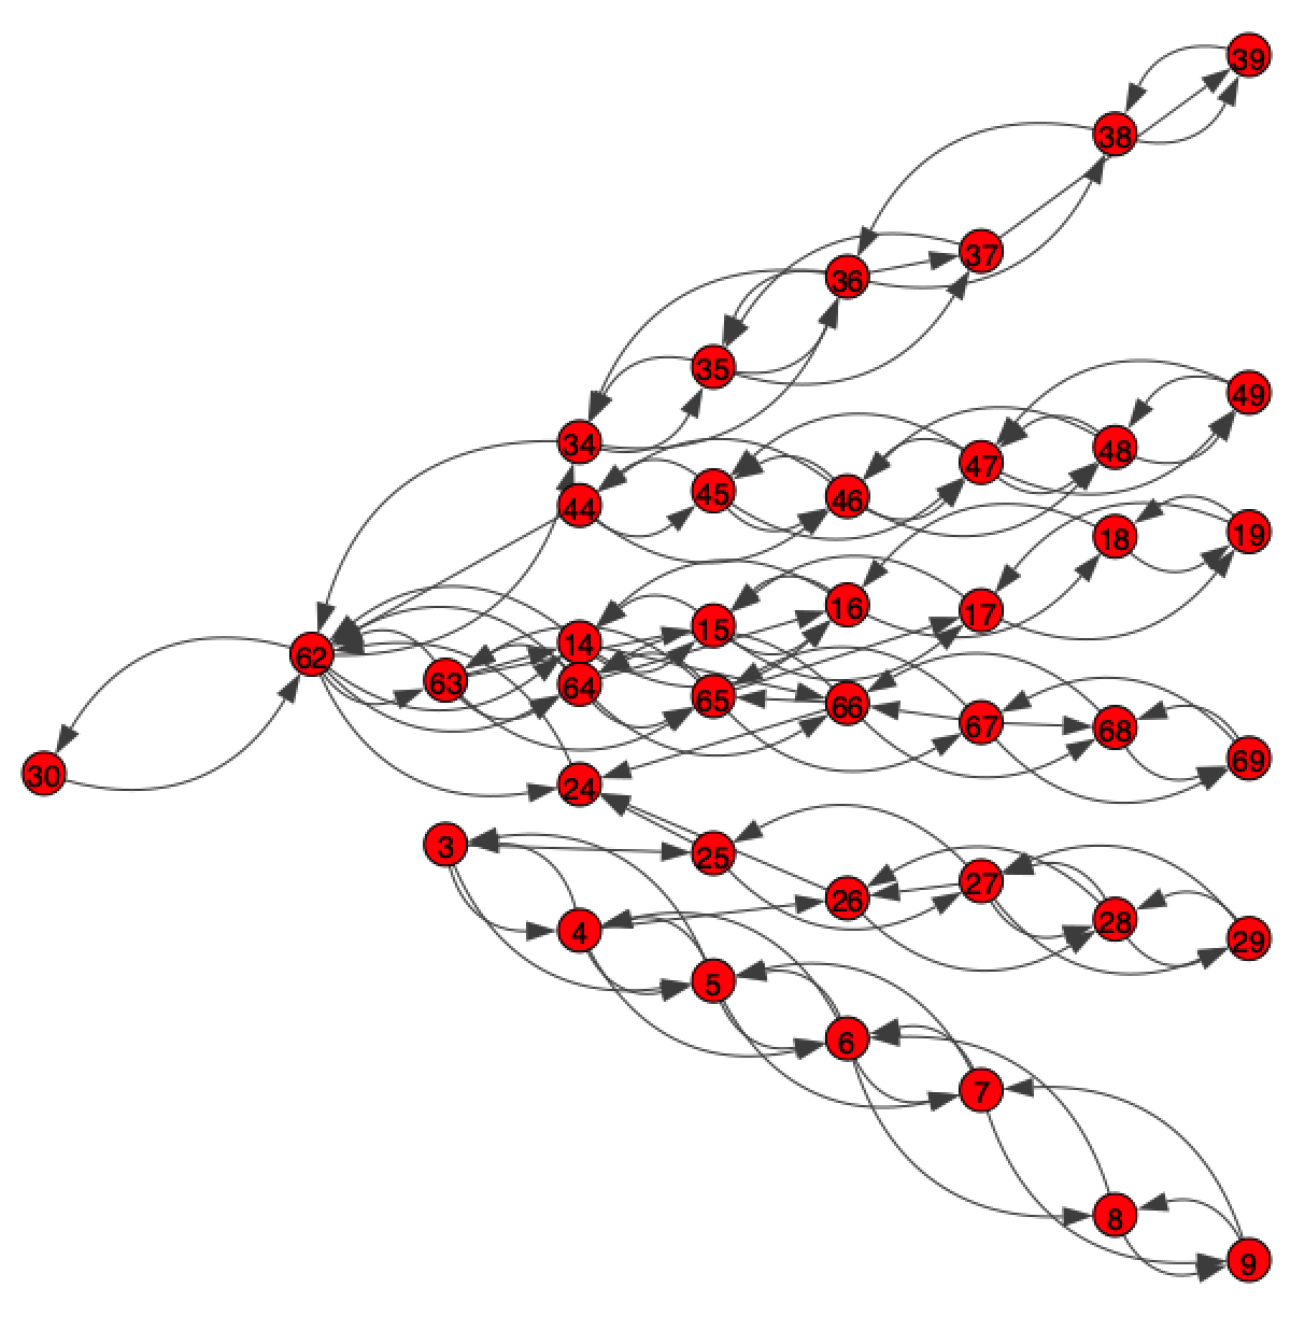
\includegraphics[width=0.45\linewidth]{images/7-results/community-detection-1.png}%
        \label{fig:community-detection-1}%
        }%
    \hfill%
    \subfloat[]{%
        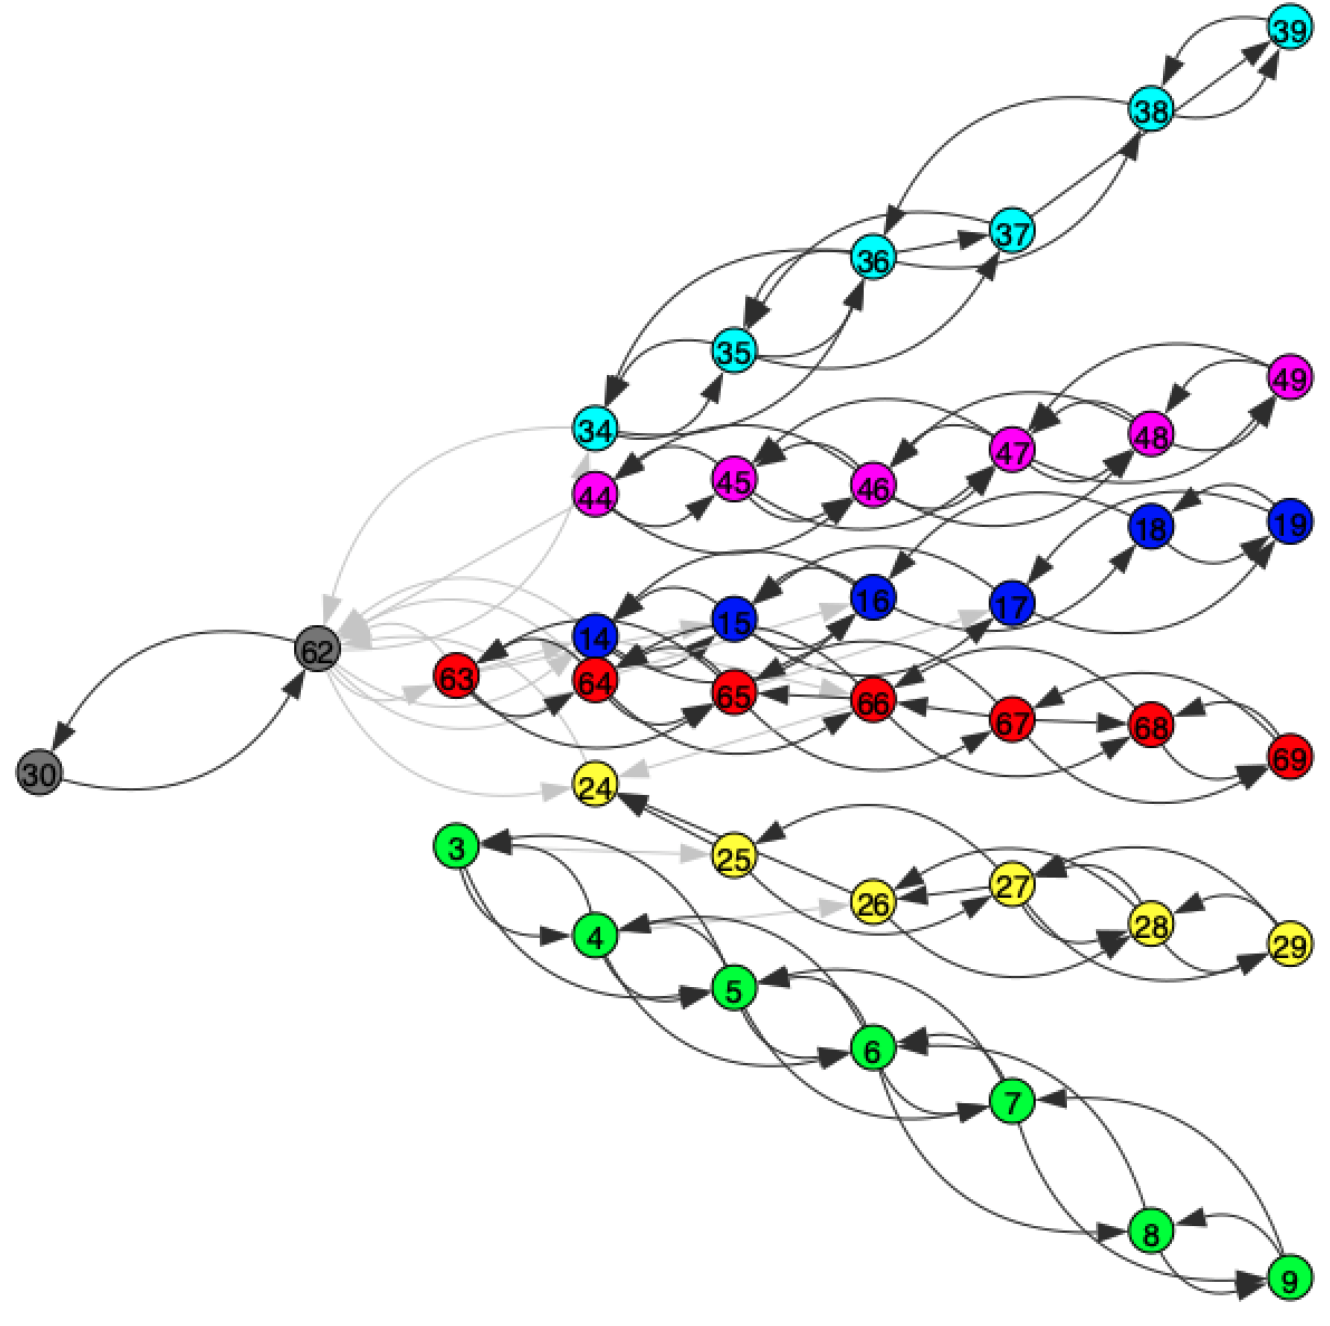
\includegraphics[width=0.45\linewidth]{images/7-results/community-detection-2.png}%
        \label{fig:community-detection-2}%
        }%
    \caption{Example application of the Community Detection algorithm applied to a small group of nodes from a TrackML event. a) Subset of nodes and edges connected as one subgraph shown in red. b) Post application of the Community Detection algorithm. Separation of the subgraph in a) into potential track candidates represented by separate colours. The faint grey edges show connections that have been deactivated through Community Detection.}
    \label{fig:community-detection}
\end{figure}

Figure \ref{fig:community-detection-1} shows a small subset of nodes from a TrackML event and its corresponding edges connected as one subgraph. The general shape of the network gives an indication that the tracks originate from the left-hand side, where the trajectories move towards the right-hand side. The results of application of Community Detection are shown in Figure \ref{fig:community-detection-2}. In this instance, the Community Detection was successful to partition the network into a total of seven subgraphs shown by separate colours. Six of these subgraphs met the criteria for a good track candidate, and a single track fragment was also formed shown by the grey subgraph containing two nodes. However upon further investigation, this procedure did not work successfully in all cases, specifically in dense environments, and the algorithm was found to not utilize node properties during network partition. Therefore, as this procedure needed further refinement, it was not implemented into the main GNN pattern recognition algorithm. 

A technique such as Community Detection is advantageous for a problem such as track splitting, as it provides fast convergence in track extraction, given that the algorithm is adapted for highly dense environments.





\section{Conclusion}

It is promising to see that the GNN algorithm works on simulated particle collision events produced by the TrackML detector, which have significant track multiplicity. The proposed GNN algorithm is successful in identifying outlier edge connections in an iterative manner, as well as successful in extracting track candidates for the endcap regions. It is an encouraging result that this methodology provides a high performance for fully contained tracks within the endcap volume, achieving 93.3\% average track reconstruction efficiency for tracks with $p_{\text{T}} >$ 1GeV averaged over 50 simulated TrackML events. The average track purity and average particle purity achieved were 99.0\% for both quantities. Overall, the application to the endcap region is highly successful.

Neighbourhood complexity is inferred by the network, this is observed as the GNN algorithm automatically initiates the pattern recognition process in regions where outlier connections are easily identifiable. The network starts with low density regions (both endcap regions) and gradually progresses towards higher density areas (the transition between the barrel and endcap layers). This shows that the GNN algorithm behaves as expected.

However the algorithm requires significant refinement and further improvement for application to the Pixel barrel region. A deeper understanding is needed in order to evaluate the behaviour of the network on the Pixel barrel region and assess the quality of its performance. Further work would include improvement of Stage 2 of the GNN algorithm in order to improve the TPR and TNR, as well as analysis of the remaining network within the barrel region.
